\documentclass[preprint,12pt]{elsarticle}

\usepackage[UTF8]{ctex}
\usepackage{graphicx}
\usepackage{booktabs}
\usepackage{threeparttable}
\usepackage{amsmath}
\usepackage{siunitx}
\usepackage[hypertexnames=false]{hyperref}
\usepackage{xurl}
\usepackage{float}
\usepackage{longtable}
\usepackage{array}

\graphicspath{{figures/}}
\biboptions{numbers,sort&compress}
\sisetup{round-mode=places,round-precision=3}

\journal{暖通空调课程设计}

\begin{document}

\begin{frontmatter}

\title{基于不同气候分区的某办公楼中央空调系统设计\\——VRF+DOAS与FCU+DOAS方案比较研究}

\author{指导教师：\quad 学生：}

\begin{highlights}
\item 以实际建筑图纸为原型构建EnergyPlus统一仿真模型，覆盖五城市$\times$三工况$\times$两系统的15组比较矩阵。
\item 先以理想负荷基线剥离气候驱动效应，再引入VRF+DOAS与FCU+DOAS方案横向对比。
\item 北方城市供热主导、南方城市制冷主导的梯度变化规律显著。
\item FCU+DOAS电耗口径的比较结论需结合锅炉燃料消耗审慎解读。
\item 补齐了FCU+DOAS方案的全年天然气消耗数据，为综合能耗评价提供完整框架。

\end{highlights}

\begin{abstract}

本课程设计以某三层办公楼为对象，完成供冷季制冷空调设计中的夏季冷负荷计算、房间级热源参数设置、新风处理和设备选型。建筑面积约1358.4\,m²，平面尺寸约32.0\,m $\times$ 14.15\,m，三层共划分为15个天正暖通计算分区，并在CLTD/CLF计算中保留50个房间的人员、照明、设备、新风和末端选型参数。设计选取沈阳、天津、成都、重庆和深圳五个城市进行比较，分析围护结构、室外温湿度和新风除湿需求对多联机和风机盘管加独立新风系统的影响。

全文采用天正暖通计算的工程设计思路：室内设计参数统一取夏季室温26\,\textcelsius、相对湿度60\%，基准新风量40\,m³/(h·人)，照明功率密度10\,W/m²，普通办公设备功率密度15\,W/m²；会议、门厅、医务、档案、卫生间和走廊等房间按功能分别修正人员密度、设备功率和新风指标。围护结构按五城市气候区差异化设置，且南方城市采用略优于参考设计的外窗遮阳和屋面保温参数，以体现本设计的节能优化取向。

计算结果表明，五城市三层办公楼设计峰值冷负荷由低到高大致为沈阳、成都、天津、深圳、重庆。重庆和深圳的新风及除湿负荷占比更高，设备选型受高温高湿和长供冷季共同约束；沈阳、天津则更强调围护保温与短时峰值冷量校核。多联机室内机按房间峰值冷负荷乘1.3安全系数选型，大房间采用多台嵌入式末端并联，每层设置独立室外机系统并校核室内外机容量配比。进一步设置新风量、室内温度、窗墙比、设备功率密度和围护遮阳的单因素灵敏度分析，用于识别影响冷源容量和新风负荷的关键参数。

\smallskip
\noindent\textbf{关键词：}制冷空调；办公建筑；冷负荷计算；供冷季；设备选型；多联机；风机盘管；独立新风

\end{abstract}

\begin{keyword}
气候分区 \sep 办公建筑 \sep 冷负荷计算 \sep VRF \sep FCU+DOAS \sep EnergyPlus \sep 课程设计
\sep Climate zone \sep Office building \sep Cooling load calculation \sep Variable refrigerant flow \sep Fan coil unit \sep Dedicated outdoor air system
\end{keyword}

\end{frontmatter}

\section{工程概况}

\subsection{建筑概况}

本课程设计以某实际办公楼工程图纸（AutoCAD 2024，天正暖通格式）为建筑原型。经DWG到DXF的几何转换与提取后，在EnergyPlus 23.2平台上构建了逐时建筑能耗仿真模型\cite{crawley2001energyplus,energyplus232docs}。该办公楼总服务建筑面积约\SI{911}{\meter^2}，共两层，均为地上建筑。建筑占地面积\SI{32.0}{\meter} $\times$ \SI{14.24}{\meter}，建筑总高度\SI{7.0}{\meter}。每层层高均为\SI{3.5}{\meter}。建筑朝向为正南北向，南向主立面宽度\SI{32.0}{\meter}。每层建筑面积均为\SI{455.7}{\meter^2}。

建筑采用钢筋混凝土框架结构，外围护结构由外墙、外窗和屋面构成。外墙采用200 mm砖墙加50 mm挤塑聚苯板（XPS）外保温构造；外窗为双层3 mm透明玻璃加12 mm空气间层的中空玻璃窗，南、北立面各均匀布置三组通高窗带（窗高\SI{3.36}{\meter}）；屋面采用XPS保温倒置式屋面。建筑的主要功能房间包括行政办公室、会议室、档案室、休息室等办公类用房。

本课程设计考虑到各房间之间的温差不显著，因此不考虑内墙、内门、内窗和楼板的负荷参与计算。空调冷负荷计算中，由于设置新风系统导入室外新风，室内维持微正压，可防止室外空气无组织渗入，因此不考虑渗透冷负荷。

\subsection{室内设计参数}

参照GB~50189-2015《公共建筑节能设计标准》\cite{gb50189}及本课程设计任务书，室内设计参数统一设置如下：

\begin{table}[tbp]
\centering
\caption{室内设计参数}
\label{tab:indoor-params}
\scriptsize
\begin{tabular}{@{}ll@{}}
\toprule
参数 & 取值 \\
\midrule
夏季室内设计温度 & \SI{26}{\degreeCelsius} \\
夏季室内设计相对湿度 & 60\% \\
冬季室内设计温度（供暖） & \SI{21}{\degreeCelsius} \\
冬季室内设计相对湿度（供暖） & 不控制 \\
人均新风量 & \SI{30}{\meter^3\per\hour}/人 \\
照明功率密度 & \SI{10}{\watt/m^2} \\
设备功率密度 & \SI{15}{\watt/m^2} \\
人员密度 & \SI{10}{\meter^2}/人 \\
人员在室时间 & \SI{10}{h}（8:00--18:00） \\
窗面积（标准） & \SI{5}{m^2} \\
门面积（标准） & \SI{1.6}{m^2} \\
\bottomrule
\end{tabular}
\end{table}

上述室内设计参数在五个城市分支中均保持一致，以消除室内参数差异对横向比较的干扰，使得城市间的负荷差异主要来源于气候条件、室外设计参数和围护结构传热特性。

\subsection{室外设计参数}

五个城市分别位于我国四个不同的建筑热工设计气候分区（严寒地区、寒冷地区、夏热冬冷地区、夏热冬暖地区），其夏季室外气象设计参数依据CSWD标准气象年数据提取，详见表\ref{tab:outdoor-params}。

\begin{table}[tbp]
\centering
\caption{五城市夏季室外设计参数}
\label{tab:outdoor-params}
\scriptsize
\begin{tabular}{@{}lccccc@{}}
\toprule
参数 & 沈阳 & 天津 & 成都 & 重庆 & 深圳 \\
\midrule
气候分区 & 严寒 & 寒冷 & \multicolumn{2}{c}{夏热冬冷} & 夏热冬暖 \\
\midrule
夏季干球温度 (\si{\degreeCelsius}) & 31.5 & 33.9 & 31.9 & 35.5 & 33.7 \\
夏季湿球温度 (\si{\degreeCelsius}) & 25.3 & 26.9 & 26.4 & 27.6 & 27.5 \\
日平均温度 (\si{\degreeCelsius}) & 27.3 & 29.4 & 27.8 & 30.7 & 29.8 \\
室外风速 (\si{m/s}) & 3.2 & 2.3 & 1.3 & 1.6 & 2.4 \\
冬季干球温度 (\si{\degreeCelsius}) & -22.0 & -9.6 & 1.3 & 3.7 & 8.4 \\
最热月平均 (\si{\degreeCelsius}) & 24.6 & 26.5 & 25.5 & 28.5 & 28.8 \\
\bottomrule
\end{tabular}
\end{table}

由表可见，从北（沈阳）到南（深圳），夏季室外设计温度总体上呈升高趋势，制冷设计条件趋于严峻；冬季室外设计温度则从\SI{-22.0}{\degreeCelsius}升至\SI{8.4}{\degreeCelsius}，供暖设计条件显著弱化。重庆夏季室外湿球计算温度最高（\SI{27.6}{\degreeCelsius}），表明其夏季高温高湿特征在五个城市中最为突出。

\subsection{围护结构节能计算参数}

依据GB~50189-2015对不同气候分区围护结构传热系数限值的要求\cite{gb50189}，本设计按四个气候分区进行围护结构差异化设定。外墙和屋面通过改变挤塑聚苯板（XPS）保温层厚度调节传热系数，外窗统一采用双层3 mm透明玻璃加12 mm空气间层的中空玻璃（$K$=2.72 \si{W\per\square\meter\per\degreeCelsius}）。各气候分区的围护结构构造层次及传热系数见表\ref{tab:envelope}。

\begin{table}[tbp]
\centering
\caption{各气候分区围护结构构造层次与热工参数（GB~50189-2015）}
\label{tab:envelope}
\scriptsize
\begin{tabular}{@{}lcccc@{}}
\toprule
围护结构 & \makecell[c]{严寒\\（沈阳）} & \makecell[c]{寒冷\\（天津）} & \makecell[c]{夏热冬冷\\（成都、重庆）} & \makecell[c]{夏热冬暖\\（深圳）} \\
\midrule
\multicolumn{5}{l}{\textbf{外墙（由外至内）}} \\
~~水泥砂浆 (mm) & 20 & 20 & 20 & 20 \\
~~XPS保温层 (mm) & 70 & 50 & 30 & 20 \\
~~砖墙 (mm) & 200 & 200 & 200 & 200 \\
~~石膏抹灰 (mm) & 20 & 20 & 20 & 20 \\
~~$K_{\mathrm{wall}}$ (\si{W/(m^2\cdot K)}) & 0.36 & 0.48 & 0.70 & 0.91 \\
~~GB限值 & $\le$0.45 & $\le$0.50 & $\le$0.80 & $\le$1.5 \\
\midrule
\multicolumn{5}{l}{\textbf{屋面（由外至内）}} \\
~~XPS保温层 (mm) & 90 & 70 & 40 & 30 \\
~~钢筋混凝土 (mm) & 200 & 200 & 200 & 200 \\
~~水泥砂浆 (mm) & 20 & 20 & 20 & 20 \\
~~$K_{\mathrm{roof}}$ (\si{W/(m^2\cdot K)}) & 0.30 & 0.38 & 0.60 & 0.75 \\
~~GB限值 & $\le$0.35 & $\le$0.45 & $\le$0.50 & $\le$0.80 \\
\midrule
\multicolumn{5}{l}{\textbf{外窗}} \\
~~构造 & \multicolumn{4}{c}{双玻+空气} \\
~~$K_{\mathrm{win}}$ (\si{W/(m^2\cdot K)}) & 2.72 & 2.72 & 2.72 & 2.72 \\
~~GB限值 & $\le$2.5 & $\le$2.7 & $\le$3.0 & $\le$4.0 \\
\bottomrule
\end{tabular}
\end{table}

本设计中，严寒地区（沈阳）的外墙和屋面保温层最厚，传热系数最低，符合严寒气候的高保温要求；夏热冬暖地区（深圳）的外墙和屋面保温层最薄，传热系数最高，反映暖热气候的适度保温要求。围护结构参数的差异化处理使得各城市的建筑负荷特征更贴近实际工程的节能设计标准\cite{xu2013hscw_energy_standard,yang2012china_north_south}。

\subsection{主要设计依据}

本课程设计的主要设计依据及参考规范如下：
\begin{itemize}
    \item 《民用建筑供暖通风与空气调节设计规范》GB~50736-2012\cite{gb50736}
    \item 《公共建筑节能设计标准》GB~50189-2015\cite{gb50189}
    \item 《多联机空调系统工程技术规程》JGJ~174-2010\cite{jgj174}
    \item 《实用供热空调设计手册》（第二版）
    \item EnergyPlus\textsuperscript{\texttrademark} 23.2 技术文档及参考指南\cite{energyplus232docs}
    \item ASHRAE Standard 90.1-2019: Energy Standard for Buildings
    \item 中国建筑科学研究院. CSWD标准气象年数据\cite{onebuilding}
\end{itemize}

\subsection{建筑热工分区与面积}

本课程设计将每层建筑平面划分为五个热工分区（thermal zones）：核心区（C）位于平面中央，不直接接触外墙，属于内区；东南西北四个周边区（S、N、W、E）各沿外墙方向布置，直接受室外气象条件影响。两层共计10个热工分区，每个分区独立进行负荷计算与空调末端选型。

建筑分区命名规则为 ZF\{层号\}\_\{方位\}，例如ZF1\_S表示一层南侧周边区，ZF2\_C表示二层核心区。

\begin{table}[tbp]
\centering
\caption{建筑各层分区面积表}
\label{tab:zone-areas}
\scriptsize
\begin{tabular}{@{}lccccc@{}}
\toprule
楼层 & 核心区 C & 南周边 S & 北周边 N & 西周边 W & 东周边 E \\
 & \si{m^2} & \si{m^2} & \si{m^2} & \si{m^2} & \si{m^2} \\
\midrule
一层（ZF1） & 174.6 & 115.2 & 115.2 & 25.3 & 25.3 \\
二层（ZF2） & 174.6 & 115.2 & 115.2 & 25.3 & 25.3 \\
\midrule
合计 & 349.2 & 230.4 & 230.4 & 50.6 & 50.6 \\
\bottomrule
\end{tabular}
\end{table}

总空调服务建筑面积为\SI{911}{\meter^2}。其中，核心区占总面积的约38.3\%，南、北周边区各占约25.3\%，东、西周边区各占约5.6\%。

\begin{figure}[htbp]
\centering
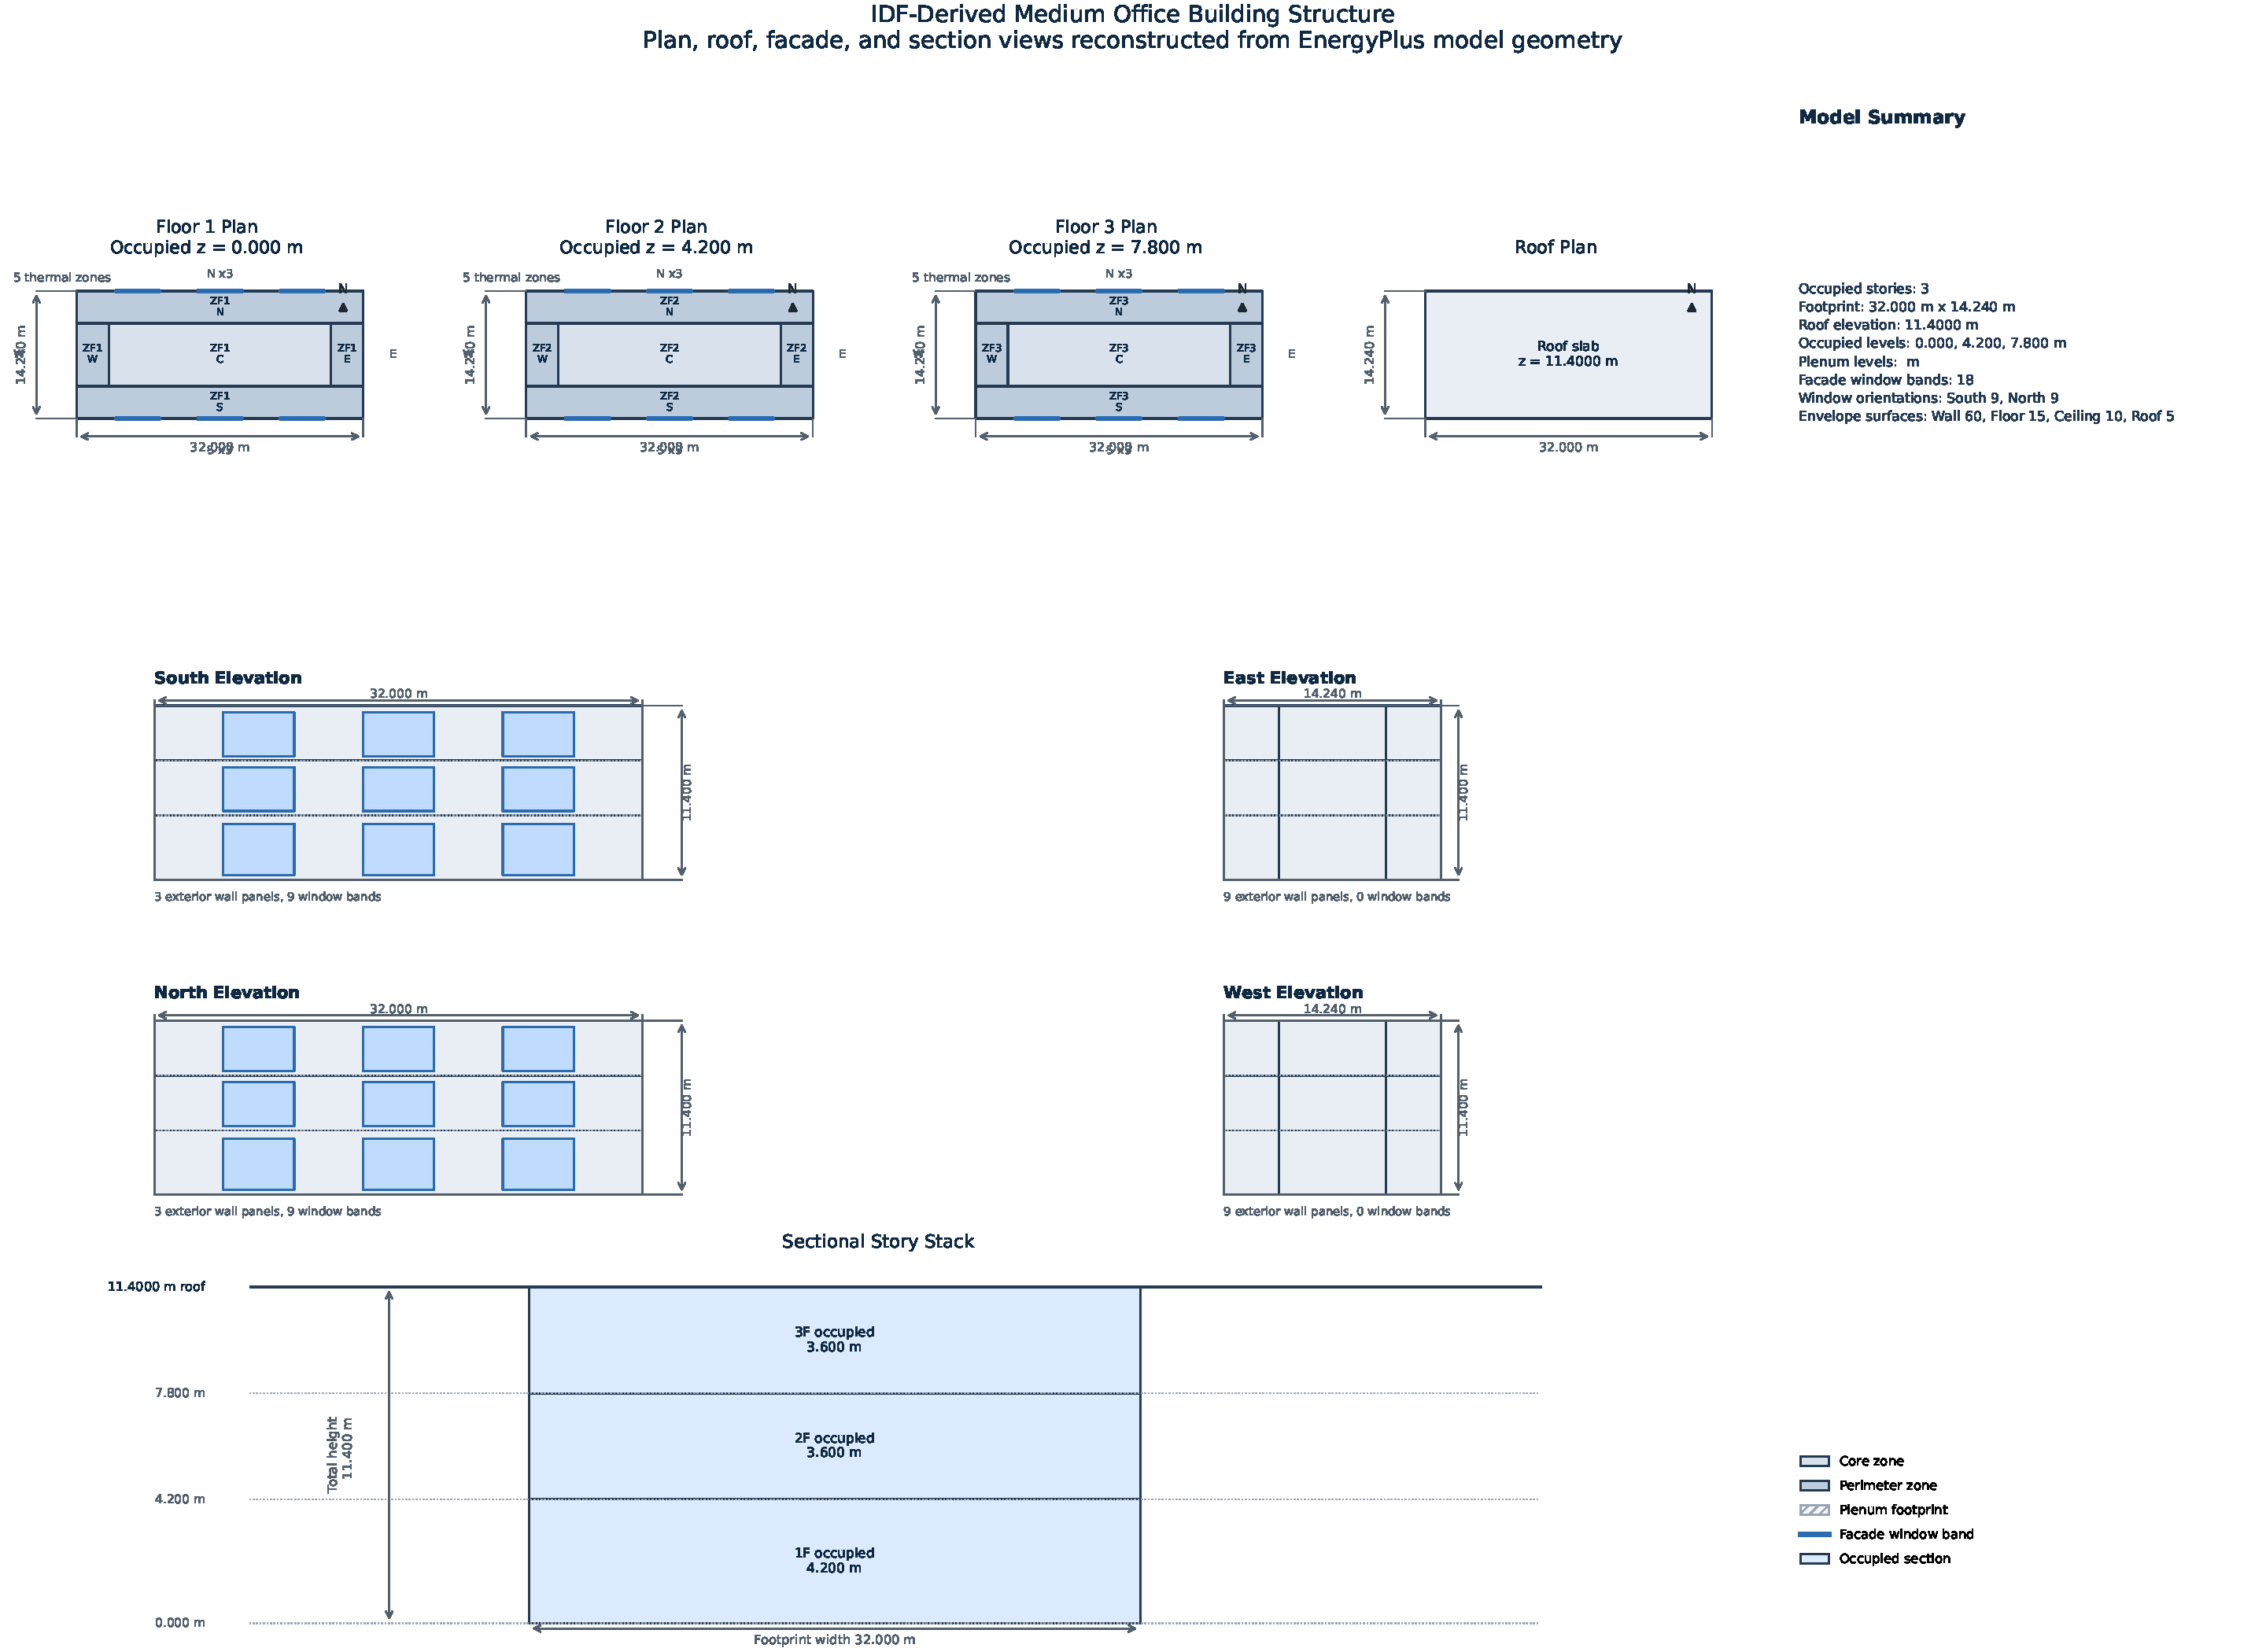
\includegraphics[width=\textwidth]{medium_office_building_model_structure.pdf}
\caption{基于实际工程图纸提取的建筑模型多视图表达，包括各层平面、屋顶平面、四向立面和纵向剖面}
\label{fig:building-structure}
\end{figure}

\subsection{冷负荷构成及计算原理}

\subsubsection{传统冷负荷系数法（CLTD/CLF法）理论基础}

暖通空调课程设计中，传统的逐时冷负荷计算通常采用冷负荷温度/冷负荷系数法（CLTD/CLF法）。本课程设计在利用EnergyPlus进行全尺度逐时仿真之前，先在此对传统手工设计方法的理论框架进行系统梳理。

\textbf{一、围护结构瞬变传热冷负荷}

外墙与屋面等不透光外围护结构由于室外气温波动和太阳辐射的联合作用，通过导热延迟和衰减后传入室内的逐时冷负荷可表示为：

\begin{equation}
Q_{\mathrm{wall}}(t)=K\cdot F\cdot\left[t_{\mathrm{lc}}(t)+t_{\mathrm{d}}-t_{\mathrm{n}}\right]
\label{eq:wall}
\end{equation}

式中：$K$为围护结构的传热系数，\si{W\per\square\meter\per\degreeCelsius}；$F$为围护结构面积，\si{\square\meter}；$t_{\mathrm{lc}}(t)$为墙体或屋面在$t$时刻的冷负荷计算温度逐时值，\si{\degreeCelsius}；$t_{\mathrm{d}}$为围护结构的地点修正系数，\si{\degreeCelsius}；$t_{\mathrm{n}}$为室内设计温度，\si{\degreeCelsius}。

\textbf{二、外窗冷负荷}

透过外窗的逐时冷负荷由温差传热部分和太阳辐射热部分叠加而成。

（1）温差传热冷负荷：

\begin{equation}
Q_{\mathrm{win,con}}(t)=K_{\mathrm{ch}}\cdot F_{\mathrm{ch}}\cdot\left[t_{\mathrm{lc}}(t)+t_{\mathrm{d}2}-t_{\mathrm{n}}\right]\cdot C_{K1}\cdot C_{K2}
\label{eq:win-con}
\end{equation}

式中：$K_{\mathrm{ch}}$为外窗传热系数，\si{W\per\square\meter\per\degreeCelsius}；$F_{\mathrm{ch}}$为外窗面积，\si{\square\meter}；$t_{\mathrm{lc}}(t)$为外窗的逐时冷负荷计算温度，\si{\degreeCelsius}；$C_{K1}$、$C_{K2}$分别为窗框类型修正系数和有内遮阳设施的传热系数修正值。

（2）太阳辐射热冷负荷：

\begin{equation}
Q_{\mathrm{win,rad}}(t)=F_{\mathrm{ch}}\cdot C_{\mathrm{s}}\cdot C_{\mathrm{n}}\cdot C_{\mathrm{a}}\cdot\left[J_{\mathrm{ch,zd}}(t)\cdot C_{\mathrm{cl,ch}}(t)+J_{\mathrm{sh,zd}}(t)\right]
\label{eq:win-rad}
\end{equation}

式中：$C_{\mathrm{s}}$为窗玻璃遮挡系数；$C_{\mathrm{n}}$为窗内遮阳设施的遮阳系数；$C_{\mathrm{a}}$为窗的有效面积系数；$J_{\mathrm{ch,zd}}(t)$为透过标准窗玻璃的太阳总辐射照度，\si{W\per\square\meter}；$C_{\mathrm{cl,ch}}(t)$为冷负荷系数。

\textbf{三、室内设备、照明与人体散热冷负荷}

（1）设备散热冷负荷：

\begin{equation}
Q_{\mathrm{equip}}(t)=N_{\mathrm{equip}}\cdot n_{1}\cdot n_{2}\cdot n_{3}\cdot CLF_{\mathrm{equip}}(t)
\label{eq:equip}
\end{equation}

式中：$N_{\mathrm{equip}}$为设备安装功率，\si{W}；$n_{1}$为同时使用系数（0.5--1.0）；$n_{2}$为安装系数（0.7--0.9）；$n_{3}$为负荷系数（0.4--0.5）；$CLF_{\mathrm{equip}}(t)$为设备散热冷负荷系数。

（2）照明得热冷负荷（以荧光灯为例）：

\begin{equation}
Q_{\mathrm{light}}(t)=\left[N_{\mathrm{light}}\cdot(1+\eta)\right]\cdot CLF_{\mathrm{light}}(t)
\label{eq:light}
\end{equation}

式中：$N_{\mathrm{light}}$为照明灯具安装功率，\si{W}；$\eta$为镇流器消耗功率系数，一般取0.2；$CLF_{\mathrm{light}}(t)$为照明冷负荷系数。

（3）人体散热冷负荷与湿负荷：

人体显热散热引起的逐时冷负荷为：

\begin{equation}
Q_{\mathrm{p,sen}}(t)=n\cdot q_{\mathrm{sen}}\cdot C_{\mathrm{r}}\cdot CLF_{\mathrm{p}}(t)
\label{eq:p-sen}
\end{equation}

人体潜热散热冷负荷为：

\begin{equation}
Q_{\mathrm{p,lat}}=n\cdot q_{\mathrm{lat}}\cdot C_{\mathrm{r}}
\label{eq:p-lat}
\end{equation}

人体散湿量为：

\begin{equation}
W_{\mathrm{p}}=n\cdot w\cdot C_{\mathrm{r}}
\label{eq:wet}
\end{equation}

式中：$n$为空调房间内的人数；$q_{\mathrm{sen}}$、$q_{\mathrm{lat}}$分别为不同室温和劳动性质时成年男子的显热和潜热散热量，\si{W}；$w$为人均散湿量，\si{g\per\hour}；$C_{\mathrm{r}}$为群集系数；$CLF_{\mathrm{p}}(t)$为人体显热散热冷负荷系数。

\textbf{四、新风冷负荷}

新风冷负荷按下式计算：

\begin{equation}
Q_{\mathrm{oa}}=L\cdot\rho_{\mathrm{w}}\cdot(I_{\mathrm{w}}-I_{\mathrm{n}})
\label{eq:oa}
\end{equation}

式中：$L$为新风量，\si{\meter^3\per\hour}；$\rho_{\mathrm{w}}$为夏季室外空调计算干球温度下的空气密度，一般取\SI{1.13}{\kg\per\cubic\meter}；$I_{\mathrm{w}}$、$I_{\mathrm{n}}$分别为室外和室内空气的焓值，\si{kJ\per\kg}。

\subsubsection{基于EnergyPlus的全尺度逐时仿真方法}

本文的实际工况仿真采用EnergyPlus 23.2平台的传导传递函数法（CTF）与房间空气热平衡法。与上述传统CLTD/CLF法以逐时系数表格手工叠加各冷热负荷成分不同，EnergyPlus在每一时间步（本文为\SI{10}{min}，输出汇总为\SI{1}{hour}）内同步求解围护结构非稳态导热、外表面辐射/对流耦合换热以及室内长波辐射、空气对流、各内热源和空调送风之间的联动热平衡。

对各理想负荷工况，输出变量为各空调分区的逐时理想送风显冷量与显热量率。将全部分区的冷/热率分别求和后，全年积分可得年冷负荷$E_{\mathrm{cool}}$和年热负荷$E_{\mathrm{heat}}$，其逐时最大值即为峰值冷负荷$Q_{\mathrm{pc}}$：

\begin{equation}
Q_{\mathrm{pc}}=\frac{1}{1000}\max_t\left(\sum_z \dot{Q}_{\mathrm{cool},z}(t)\right)
\label{eq:Qpc}
\end{equation}

\begin{equation}
q_{\mathrm{pc}}=\frac{1000\cdot Q_{\mathrm{pc}}}{A_{\mathrm{f}}}
\label{eq:qpc}
\end{equation}

对两类实际空调系统（VRF+DOAS、FCU+DOAS），年空调电耗$E_{\mathrm{elec}}$来自系统输出计量（Electricity:HVAC），其面积归一化指标定义为：

\begin{equation}
I_{\mathrm{elec}}=\frac{E_{\mathrm{elec}}}{A_{\mathrm{f}}}
\label{eq:Ielec}
\end{equation}

需要指出，EnergyPlus的Conduction Transfer Function方法虽然在数值层面上与CLTD/CLF以相变延迟和衰减表示的物理概念方法不同，但二者对于各热源成分在全天内的物理积蓄与逐时释放关系的描述具有本质上的一致性\cite{crawley2001energyplus,wu2019china_cooling_load}。传统CLTD/CLF设计法是理解仿真负荷波动特性的理论和实际方法学基础。

\subsection{空调系统方案概述}

\subsubsection{VRF+DOAS方案}

变制冷剂流量多联机配独立新风系统（VRF+DOAS）方案由集中设置的VRF室外机、各空调分区的直接膨胀式室内末端设备以及带全热回收转轮的新风处理系统组成\cite{aynur2010vrf_desiccant,kanisanchez2017vrf_whole_building}。室外机安装于屋顶机械平台，通过制冷剂管道竖向连接各层终端。新风由屋顶DOAS空气处理机组集中处理后，经竖向风道输送至各层分区，经风管支路与室内回风混合后送入各空调分区。

每层5个空调分区各设置一台VRF末端设备（变制冷剂流量末端），两层共计10台末端。系统采用一台公用的VRF热泵室外机，室外机设计制冷/制热容量由自动选型确定。

\begin{figure}[htbp]
\centering
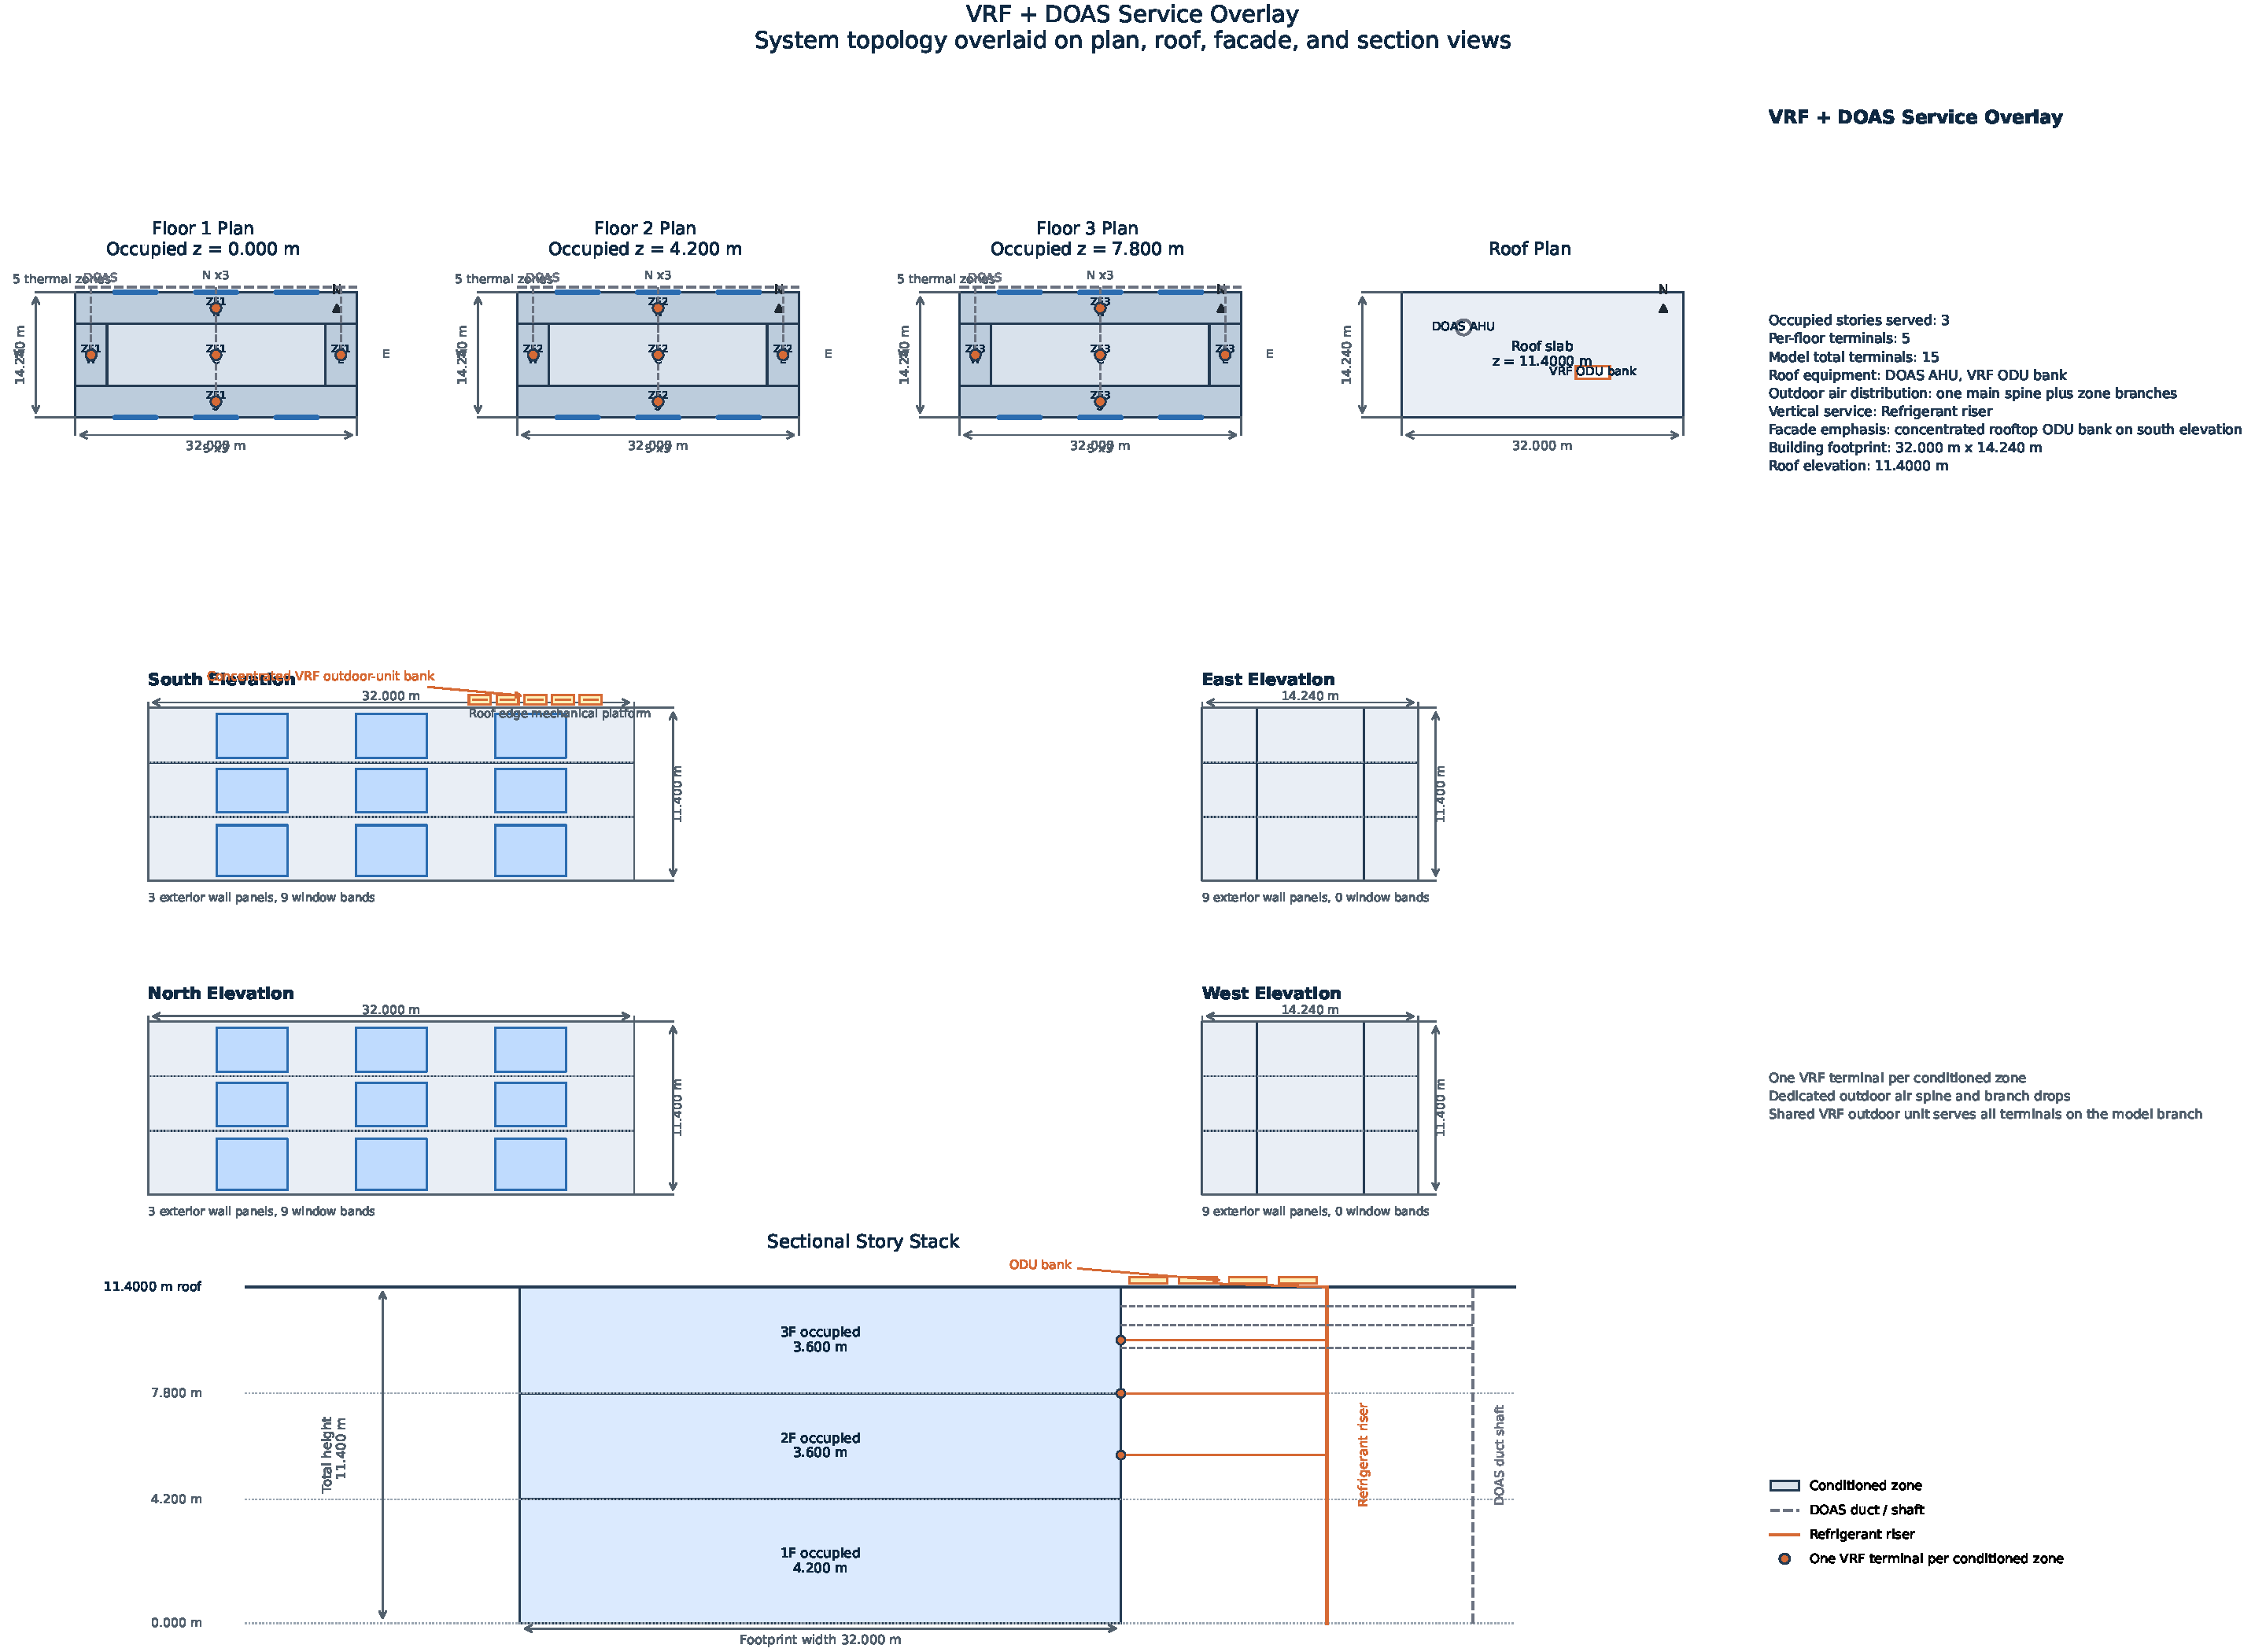
\includegraphics[width=\textwidth]{medium_office_typical_floor_vrf_doas.pdf}
\caption{VRF+DOAS方案在建筑多视图底图上的系统组织表达，突出屋顶室外机集中布置与冷媒竖向服务关系}
\label{fig:vrf-structure}
\end{figure}

\subsubsection{FCU+DOAS方案}

风机盘管配独立新风系统（FCU+DOAS）方案由四管制风机盘管末端、集中冷冻水系统（含螺杆式冷水机组与冷却塔）、集中热水系统（含燃气锅炉）以及独立新风处理系统组成。每层5个分区各设置一台四管制风机盘管末端，通过冷冻水和热水供回水立管分别与集中冷热源站连接。新风系统与VRF方案采用相同的DOAS配置，由屋顶新风机组集中处理后输送至各分区。

该方案包含两条集中水系统环路：冷冻水环路（供回水设计温度7/12\si{\degreeCelsius}）和热水环路（供回水设计温度82/60\si{\degreeCelsius}）。冷水机组和锅炉的容量均由自动选型确定。

\begin{figure}[htbp]
\centering
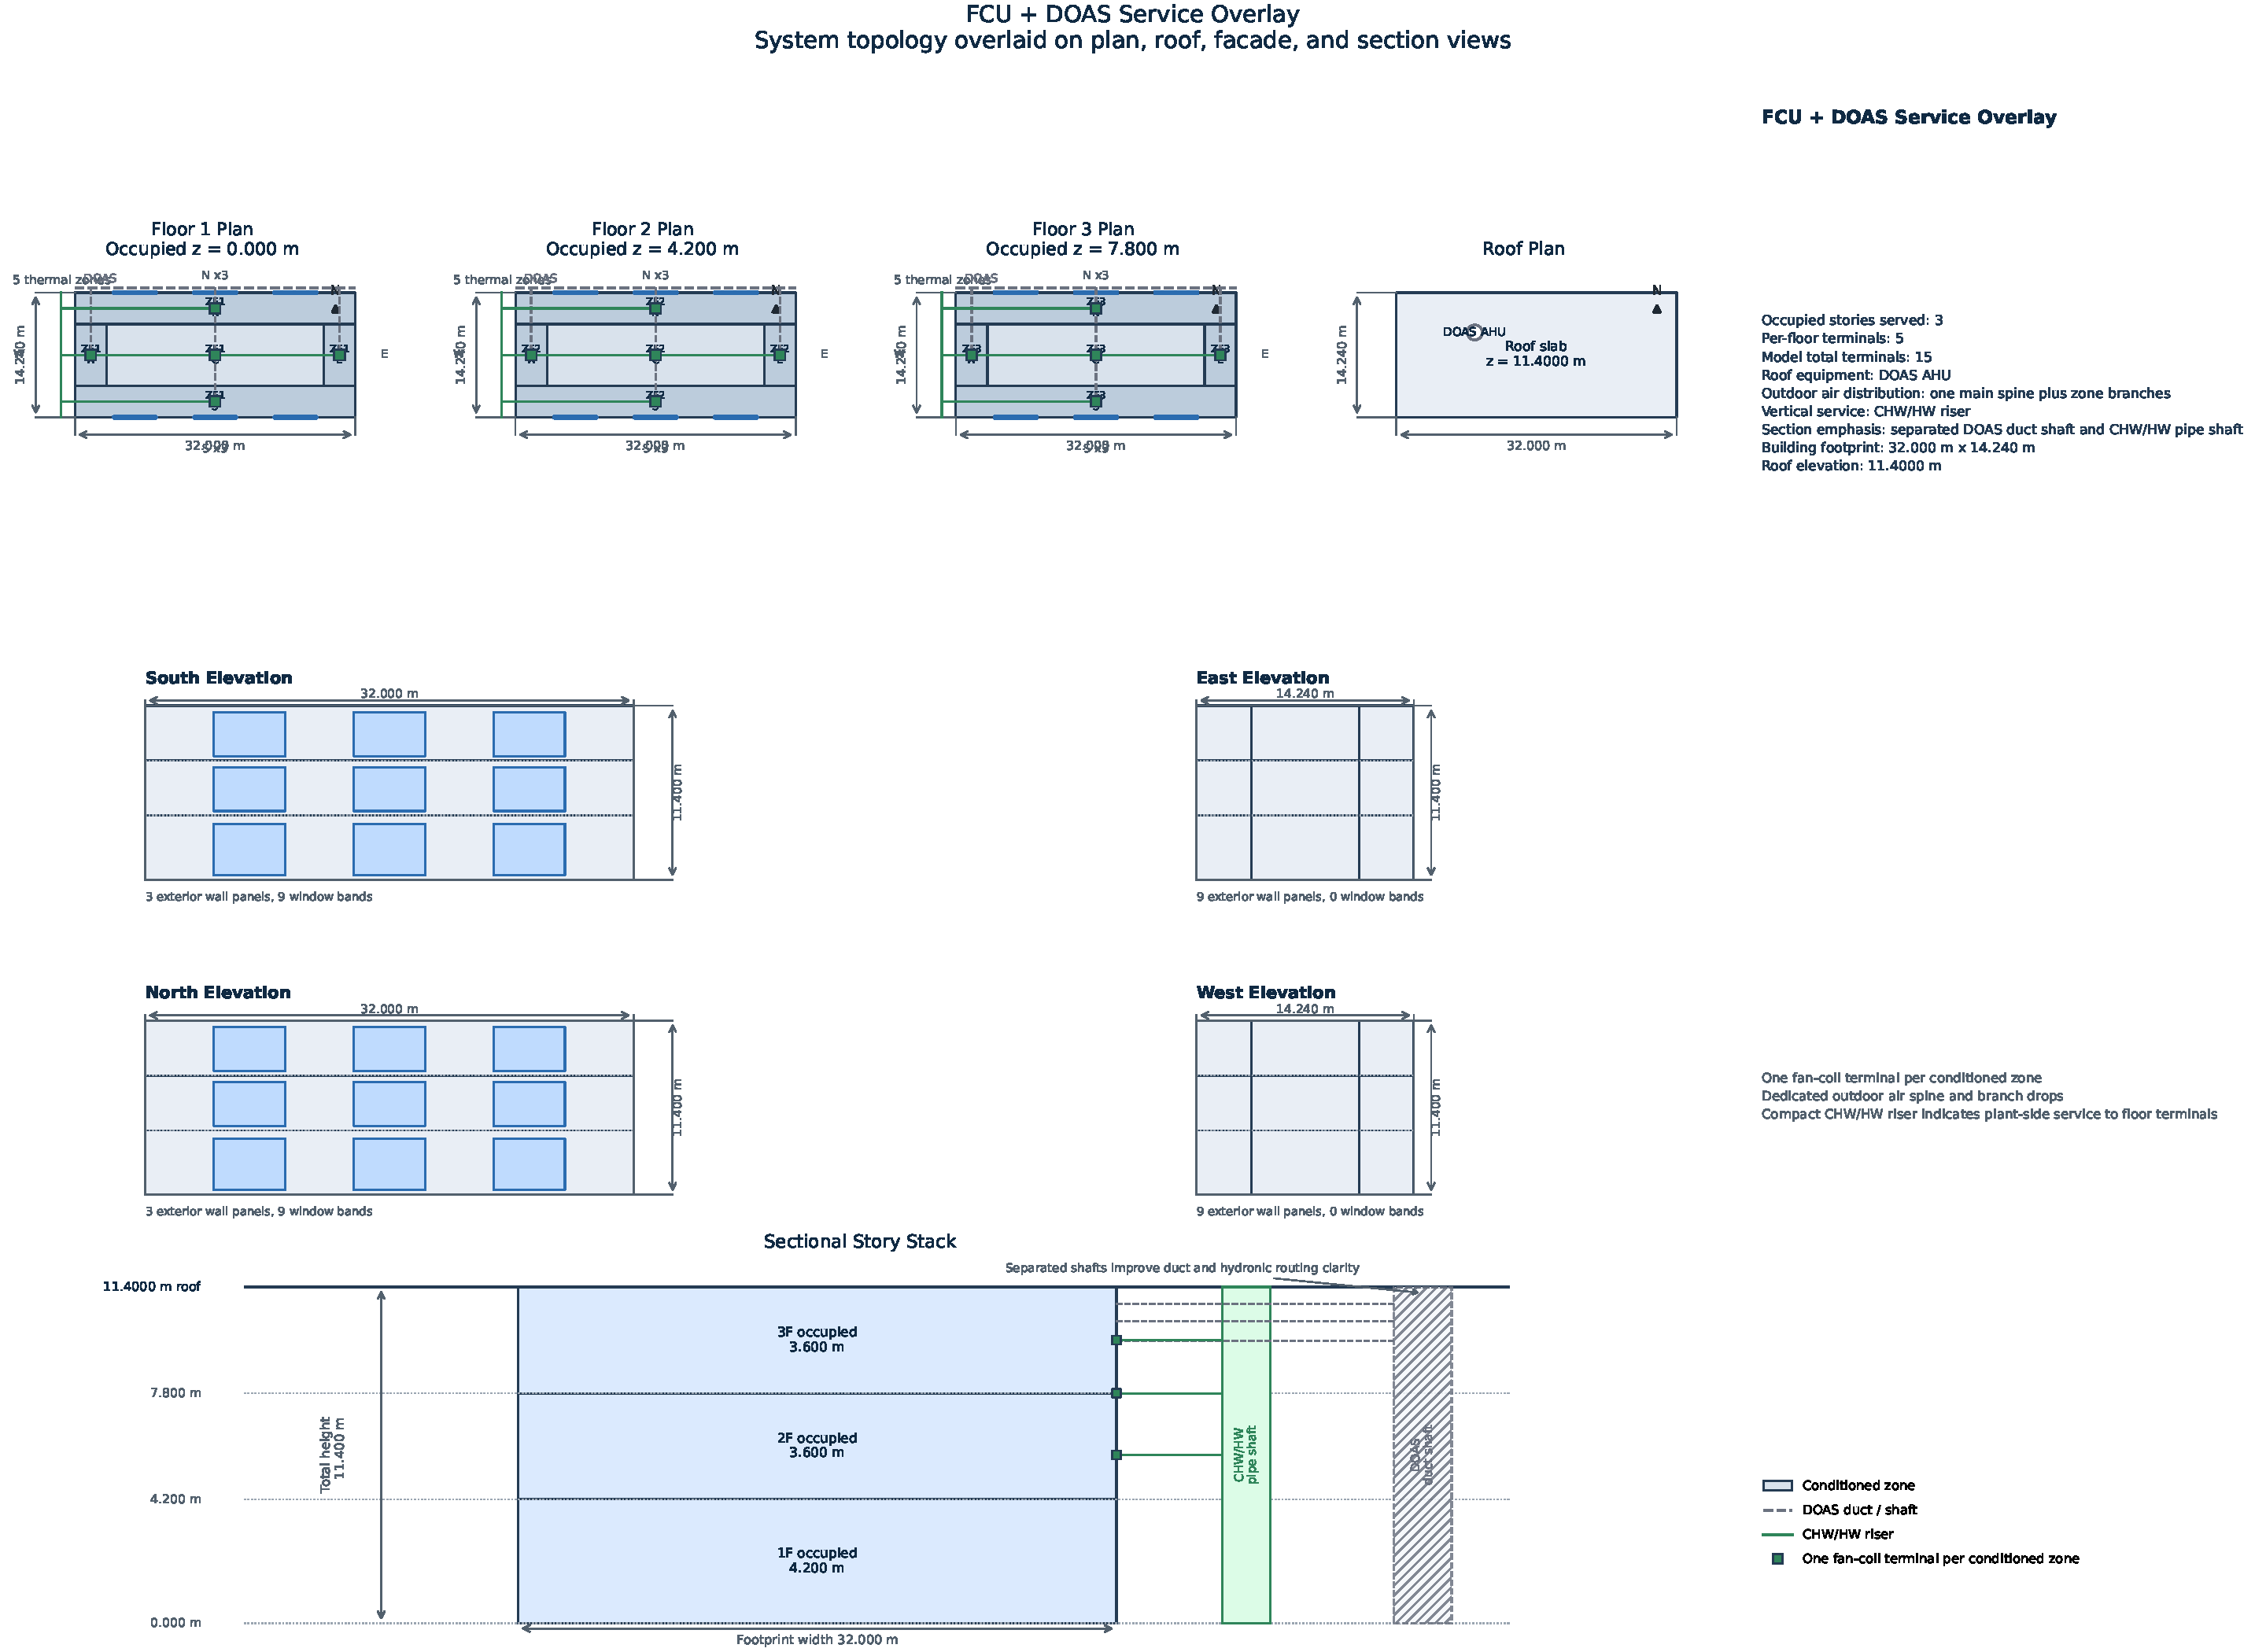
\includegraphics[width=\textwidth]{medium_office_typical_floor_fcu_doas.pdf}
\caption{FCU+DOAS方案在建筑多视图底图上的系统组织表达，突出独立新风竖井与冷热水管井的分离布置}
\label{fig:fcu-structure}
\end{figure}

两类系统方案的空调服务分区数量相同（均为10个）、设计新风量一致（约\SI{0.783}{\meter^3\per\second}，即\SI{2819}{\meter^3\per\hour}）、围护结构和室内设计参数完全相同。因此，本文的比较实质上是在”相同建筑载体、相同负荷边界”下对两类系统拓扑结构及运行性能的横向分析。

\section{沈阳多联机及风机盘管系统设计}

本章以沈阳（严寒地区）为目标城市，给出该地区的负荷计算提取结果及VRF+DOAS和FCU+DOAS两方案的设备选型结果。沈阳属于建筑热工设计气候分区中的严寒A区，冬季漫长且严寒，夏季相对短促而温和。该城市是本文五个城市中供暖需求最强的代表性样本。

\subsection{室外设计参数}

沈阳位于我国东北地区，属严寒气候。其夏季室外气象设计参数（CSWD气象年数据）为：夏季空调室外干球计算温度\SI{31.5}{\degreeCelsius}，夏季空调室外湿球计算温度\SI{25.3}{\degreeCelsius}，夏季空调室外计算日平均温度\SI{27.3}{\degreeCelsius}，夏季室外平均风速\SI{3.2}{\meter\per\second}。冬季空调室外干球计算温度为\SI{-22.0}{\degreeCelsius}，为五城市中最低值。全年最热月平均温度为\SI{24.6}{\degreeCelsius}，也是五城市中最低值，表明沈阳夏季制冷负荷峰值有限但冬季供暖与过渡季保温需求突出。

\subsection{建筑概况}

同第一章详述。室内设计参数与围护结构参数参见第一章表\ref{tab:indoor-params}与表\ref{tab:envelope}。建筑共2层10个热工分区，空调服务面积\SI{911}{\meter^2}。

\subsection{理想负荷计算结果}

由EnergyPlus理想负荷工况仿真提取得到的负荷计算及两类系统方案比较结果见表\ref{tab:shenyang-ideal}。

\begin{table}[tbp]
\centering
\caption{沈阳负荷计算与系统方案比较结果}
\label{tab:shenyang-ideal}
\scriptsize
\begin{minipage}[t]{0.42\textwidth}
\centering
\textbf{（a）理想负荷工况结果}\\[3pt]
\begin{tabular}{@{}lr@{}}
\toprule
指标 & 数值 \\
\midrule
$Q_{\mathrm{pc}}$ (kW) & 10.00 \\
$q_{\mathrm{pc}}$ (W/m$^{2}$) & 7.31 \\
$E_{\mathrm{cool}}$ (kWh) & 8814 \\
$E_{\mathrm{heat}}$ (kWh) & 203489 \\
$E_{\mathrm{total}}$ (kWh) & 212303 \\
$E/A_{\mathrm{f}}$ (kWh/m$^{2}$) & 232.95 \\
\bottomrule
\end{tabular}
\end{minipage}%
\hfill%
\begin{minipage}[t]{0.54\textwidth}
\centering
\textbf{（b）两类系统比较}\\[3pt]
\begin{tabular}{@{}lcc@{}}
\toprule
指标 & VRF+DOAS & FCU+DOAS \\
\midrule
设计冷量 (kW) & 35.60 & 54.71 \\
设计热量 (kW) & 35.60 & 57.38 \\
年电耗 (kWh) & 54889 & 4455 \\
电耗强度 (kWh/m$^{2}$) & 60.25 & 4.89 \\
\bottomrule
\end{tabular}
\end{minipage}
\end{table}

沈阳的峰值冷负荷为五城市中最低（\SI{10.00}{\kilo\watt}），但年热负荷为五城市中最高（\SI{203489}{\kilo\watt\hour}），年总单位面积负荷也是最高（\SI{232.95}{\kilo\watt\hour\per\square\meter}）。年热负荷约为年冷负荷的23.1倍，供暖需求在该地区占据绝对主导地位。

\subsection{空调系统方案比较}

在沈阳严寒气候条件下，VRF+DOAS的年空调电耗为\SI{54889}{\kilo\watt\hour}，电耗强度\SI{60.25}{\kilo\watt\hour\per\square\meter}，为五城市中最高的VRF电耗强度。这主要归因于沈阳漫长的供暖季中VRF热泵需要持续运行以满足供热需求，其压缩机在低温工况下的性能系数（COP）较低。FCU+DOAS的电耗强度仅为\SI{4.89}{\kilo\watt\hour\per\square\meter}，但需注意其供热主要依赖燃气锅炉（设计热量\SI{57.38}{\kilo\watt}），锅炉燃气消耗（\SI{85044}{\kilo\watt\hour}，折合能耗强度\SI{93.33}{\kilo\watt\hour\per\square\meter}）未计入此电耗口径。

沈阳FCU方案中，冷水机组设计冷量（\SI{54.71}{\kilo\watt}）高于VRF室外机设计冷量（\SI{35.60}{\kilo\watt}），而锅炉设计热量（\SI{57.38}{\kilo\watt}）约为VRF设计热量（\SI{35.60}{\kilo\watt}）的1.61倍。这表明在严寒地区，FCU+DOAS方案通过集中冷热源配置提供了更高的容量储备，但相应地增加了设备占地和系统复杂度。

\section{天津多联机及风机盘管系统设计}

本章以天津（寒冷地区）为目标城市。天津属于建筑热工设计气候分区中的寒冷B区，冬季较长且干冷，夏季炎热。该城市是本文中代表华北沿海寒冷气候的典型样本。

\subsection{室外设计参数}

天津夏季室外气象设计参数（CSWD气象年数据）为：夏季空调室外干球计算温度\SI{33.9}{\degreeCelsius}，夏季空调室外湿球计算温度\SI{26.9}{\degreeCelsius}，夏季空调室外计算日平均温度\SI{29.4}{\degreeCelsius}，夏季室外平均风速\SI{2.3}{\meter\per\second}。冬季空调室外干球计算温度为\SI{-9.6}{\degreeCelsius}。天津夏季干球温度在五城市中处于中间偏高水平，冬季温度则介于严寒区沈阳与南方城市之间，呈现典型的“冷热并重”过渡型气候特征。

\subsection{建筑概况}

同第一章详述。

\subsection{理想负荷计算结果}

\begin{table}[tbp]
\centering
\caption{天津负荷计算与系统方案比较结果}
\label{tab:tianjin-ideal}
\scriptsize
\begin{minipage}[t]{0.42\textwidth}
\centering
\textbf{（a）理想负荷工况结果}\\[3pt]
\begin{tabular}{@{}lr@{}}
\toprule
指标 & 数值 \\
\midrule
$Q_{\mathrm{pc}}$ (kW) & 17.05 \\
$q_{\mathrm{pc}}$ (W/m$^{2}$) & 12.47 \\
$E_{\mathrm{cool}}$ (kWh) & 13486 \\
$E_{\mathrm{heat}}$ (kWh) & 169458 \\
$E_{\mathrm{total}}$ (kWh) & 182944 \\
$E/A_{\mathrm{f}}$ (kWh/m$^{2}$) & 200.74 \\
\bottomrule
\end{tabular}
\end{minipage}%
\hfill%
\begin{minipage}[t]{0.54\textwidth}
\centering
\textbf{（b）两类系统比较}\\[3pt]
\begin{tabular}{@{}lcc@{}}
\toprule
指标 & VRF+DOAS & FCU+DOAS \\
\midrule
设计冷量 (kW) & 41.70 & 73.79 \\
设计热量 (kW) & 41.70 & 47.56 \\
年电耗 (kWh) & 54842 & 4381 \\
电耗强度 (kWh/m$^{2}$) & 60.20 & 4.81 \\
\bottomrule
\end{tabular}
\end{minipage}
\end{table}

天津理想负荷结果的显著特点是：峰值冷负荷为\SI{17.05}{\kilo\watt}，明显高于沈阳（\SI{10.00}{\kilo\watt}），但低于南方城市。年热负荷为\SI{169458}{\kilo\watt\hour}，仍占年总负荷的约92.6\%，表明供暖需求在天津仍占据主导地位。年冷负荷为\SI{13486}{\kilo\watt\hour}，约为年热负荷的8.0\%。

\subsection{空调系统方案比较}

天津VRF+DOAS的年电耗强度为\SI{60.20}{\kilo\watt\hour\per\square\meter}，略低于沈阳（\SI{60.25}{\kilo\watt\hour\per\square\meter}），反映出较温和的冬季使VRF热泵在供热工况下的运行时间有所减少。FCU+DOAS电耗强度为\SI{4.81}{\kilo\watt\hour\per\square\meter}，其年度天然气消耗为\SI{70174}{\kilo\watt\hour}（强度为\SI{77.03}{\kilo\watt\hour\per\square\meter}）。

天津FCU方案中，冷水机组设计冷量（\SI{73.79}{\kilo\watt}）与锅炉设计热量（\SI{47.56}{\kilo\watt}）之比约为1.55:1，与沈阳（冷热比约0.95:1，即54.71/57.38）形成对比，体现从北向南冷热需求量此消彼长的趋势。VRF方案的设计冷/热量均为\SI{41.70}{\kilo\watt}，位于五城市的中间水平。

\section{成都多联机及风机盘管系统设计}

本章以成都（夏热冬冷地区）为目标城市。成都位于四川盆地，属于建筑热工设计气候分区中的夏热冬冷A区，夏季炎热、冬季湿冷，全年相对湿度较高。该城市在本文中代表内陆盆地型夏热冬冷气候特征。

\subsection{室外设计参数}

成都夏季室外气象设计参数（CSWD气象年数据）为：夏季空调室外干球计算温度\SI{31.9}{\degreeCelsius}，夏季空调室外湿球计算温度\SI{26.4}{\degreeCelsius}，夏季空调室外计算日平均温度\SI{27.8}{\degreeCelsius}，夏季室外平均风速\SI{1.3}{\meter\per\second}。冬季空调室外干球计算温度为\SI{1.3}{\degreeCelsius}。成都夏季室外风速为五城市中最低（\SI{1.3}{\meter\per\second}），这与盆地的静风气候特征一致。

\subsection{建筑概况}

同第一章详述。

\subsection{理想负荷计算结果}

\begin{table}[tbp]
\centering
\caption{成都负荷计算与系统方案比较结果}
\label{tab:chengdu-ideal}
\scriptsize
\begin{minipage}[t]{0.42\textwidth}
\centering
\textbf{（a）理想负荷工况结果}\\[3pt]
\begin{tabular}{@{}lr@{}}
\toprule
指标 & 数值 \\
\midrule
$Q_{\mathrm{pc}}$ (kW) & 13.00 \\
$q_{\mathrm{pc}}$ (W/m$^{2}$) & 9.51 \\
$E_{\mathrm{cool}}$ (kWh) & 12437 \\
$E_{\mathrm{heat}}$ (kWh) & 92799 \\
$E_{\mathrm{total}}$ (kWh) & 105236 \\
$E/A_{\mathrm{f}}$ (kWh/m$^{2}$) & 115.47 \\
\bottomrule
\end{tabular}
\end{minipage}%
\hfill%
\begin{minipage}[t]{0.54\textwidth}
\centering
\textbf{（b）两类系统比较}\\[3pt]
\begin{tabular}{@{}lcc@{}}
\toprule
指标 & VRF+DOAS & FCU+DOAS \\
\midrule
设计冷量 (kW) & 45.80 & 56.70 \\
设计热量 (kW) & 45.80 & 50.16 \\
年电耗 (kWh) & 44503 & 4227 \\
电耗强度 (kWh/m$^{2}$) & 48.85 & 4.64 \\
\bottomrule
\end{tabular}
\end{minipage}
\end{table}

成都年总单位面积负荷为\SI{115.47}{\kilo\watt\hour\per\square\meter}，是五城市中最低值。年热负荷（\SI{92799}{\kilo\watt\hour}）约为年冷负荷（\SI{12437}{\kilo\watt\hour}）的7.5倍。成都的峰值冷负荷（\SI{13.00}{\kilo\watt}）低于天津（\SI{17.05}{\kilo\watt}），这一结果与成都夏季室外干球温度（\SI{31.9}{\degreeCelsius}）低于天津（\SI{33.9}{\degreeCelsius}）的趋势一致。盆地地形和较高的云量减少了成都的太阳辐射得热量，从而抑制了制冷高峰负荷。

\subsection{空调系统方案比较}

成都VRF+DOAS的年电耗强度为\SI{48.85}{\kilo\watt\hour\per\square\meter}，已显著低于北方两城市，以制冷为主的全年运行模式有效降低了热泵供热工况的低温低效运行时间。FCU+DOAS电耗强度为\SI{4.64}{\kilo\watt\hour\per\square\meter}，其年度天然气消耗为\SI{68152}{\kilo\watt\hour}（强度为\SI{74.81}{\kilo\watt\hour\per\square\meter}）。

成都FCU方案中，冷水机组设计冷量（\SI{56.70}{\kilo\watt}）与锅炉设计热量（\SI{50.16}{\kilo\watt}）之比为1.13:1，冷源容量首次超过了热源容量，标志着从供暖主导型向制冷主导型的过渡。VRF方案的设计冷/热量均为\SI{45.80}{\kilo\watt}。

\section{重庆多联机系统设计}

本章按三层办公楼房间级参数完成重庆工况下的夏季冷负荷计算和VRF设备选型。重庆属于夏热冬冷高湿地区，设计重点为高温高湿叠加，峰值冷量和除湿压力最大。计算模型采用50个房间级热源参数和15个天正暖通计算分区，房间热源参数包括人员、照明、设备、新风和外窗朝向。

\subsection{室外设计参数与围护结构}

重庆室内设计参数统一取\SI{26}{\degreeCelsius}、相对湿度60\%，基准新风量40~m$^3$/(h$\cdot$人)。围护结构采用本设计的优化参数，和参考设计相比，南方城市强化遮阳控制，北方城市强化保温控制。

\begin{table}[!htbp]
\centering
\caption{重庆室外设计参数与围护结构参数}
\label{tab:chongqing-envelope}
\zihao{-5}
\begin{tabular}{@{}lccccccc@{}}
\toprule
城市 & 干球温度 & 湿球温度 & 日平均温度 & 外墙K & 屋面K & 外窗K & SC \\
 & \si{\degreeCelsius} & \si{\degreeCelsius} & \si{\degreeCelsius} & \si{W/(m^2\cdot K)} & \si{W/(m^2\cdot K)} & \si{W/(m^2\cdot K)} & -- \\
\midrule
重庆 & 35.5 & 27.6 & 30.7 & 0.72 & 0.52 & 2.50 & 0.34 \\
\bottomrule
\end{tabular}
\end{table}

\subsection{房间级冷负荷计算结果}

重庆全楼峰值冷负荷为\SI{150.48}{kW}，峰值冷负荷指标为\SI{110.8}{W/m^2}，峰值时刻为14:00。其中室内侧负荷为\SI{79.93}{kW}，新风冷负荷为\SI{70.55}{kW}，新风占比约46.9\%。主要高负荷房间见表~\ref{tab:chongqing-top-rooms}。

\begin{table}[!htbp]
\centering
\caption{重庆主要房间峰值冷负荷与热源参数}
\label{tab:chongqing-top-rooms}
\zihao{-5}
\begin{tabular}{@{}cccccccc@{}}
\toprule
楼层 & 房间编号 & 房间名称 & 面积 & 人数 & 新风量 & 峰值冷负荷 & 新风冷负荷 \\
 & -- & -- & \si{m^2} & 人 & \si{m^3/h} & \si{kW} & \si{kW} \\
\midrule
1 & 1001 & 外贸办公室 & 78.5 & 14 & 630 & 11.99 & 6.13 \\
2 & 2008 & 办公大厅 & 54.9 & 10 & 450 & 8.78 & 4.38 \\
3 & 3007 & 会客室 & 37.8 & 11 & 440 & 8.04 & 4.28 \\
3 & 3013 & 小型会议室 & 38.6 & 11 & 440 & 7.50 & 4.28 \\
1 & 1012 & 值班室 & 54.1 & 8 & 320 & 7.06 & 3.11 \\
1 & 1008 & 陈列室 & 73.9 & 7 & 245 & 6.76 & 2.38 \\
1 & 1011 & 接待大厅 & 61.0 & 7 & 245 & 6.17 & 2.38 \\
2 & 2001 & 办公室1 & 39.3 & 6 & 240 & 5.60 & 2.33 \\
3 & 3018 & 办公茶歇区 & 25.9 & 7 & 280 & 4.71 & 2.73 \\
3 & 3017 & 办公室4 & 36.1 & 5 & 200 & 4.54 & 1.95 \\
\bottomrule
\end{tabular}
\end{table}

\subsection{VRF室内外机选型与容量配比}

室内机按房间峰值冷负荷乘1.3安全系数选型，普通办公、会议和会客房间优先采用四面出风嵌入式室内机，卫生间、走廊、档案和储藏类房间采用薄型风管或壁挂式末端。重庆共配置48台室内机，室内机名义制冷量合计\SI{243.1}{kW}。每层设置一个室外机系统，容量配比范围为114.0\%--117.9\%，满足JGJ~174-2010中50\%--130\%的组合率要求。

\begin{table}[!htbp]
\centering
\caption{重庆各楼层VRF室内外机容量配比}
\label{tab:chongqing-vrf-ratio}
\zihao{-5}
\begin{tabular}{@{}ccccccc@{}}
\toprule
楼层 & 室内机台数 & 室内容量 & 室外机型号 & 室外机台数 & 室外容量 & 配比 \\
 & 台 & \si{kW} & -- & 台 & \si{kW} & \% \\
\midrule
1 & 12 & 70.1 & VRF-O615 & 1 & 61.5 & 114.0 \\
2 & 16 & 78.7 & VRF-O680 & 1 & 68.0 & 115.7 \\
3 & 20 & 94.3 & VRF-O800 & 1 & 80.0 & 117.9 \\
\bottomrule
\end{tabular}
\end{table}

从负荷组成看，重庆的新风冷负荷占比为46.9\%，该比例直接影响DOAS或新风预处理设备的容量。若施工图阶段采用厂家样本深化，应优先复核高负荷房间的室内机布置、冷媒管长修正和室外机通风散热条件。

\section{深圳多联机及风机盘管系统设计}

本章以深圳（夏热冬暖地区）为目标城市。深圳位于华南沿海，属于建筑热工设计气候分区中的夏热冬暖B区，全年温暖湿润，冬季短促温和，夏季漫长酷热。该城市在本文中代表华南沿海纯制冷导向型气候的极端样本。

\subsection{室外设计参数}

深圳夏季室外气象设计参数（CSWD气象年数据）为：夏季空调室外干球计算温度\SI{33.7}{\degreeCelsius}，夏季空调室外湿球计算温度\SI{27.5}{\degreeCelsius}，夏季空调室外计算日平均温度\SI{29.8}{\degreeCelsius}，夏季室外平均风速\SI{2.4}{\meter\per\second}。冬季空调室外干球计算温度为\SI{8.4}{\degreeCelsius}，为五城市中最高值，表明深圳的冬季供暖需求在五个城市中最为有限。深圳全年最热月平均温度（\SI{28.8}{\degreeCelsius}）为五城市中最高，全年制冷季极长，是本文代表“以制冷为全年主导”的典型城市。

\subsection{建筑概况}

同第一章详述。

\subsection{理想负荷计算结果}

\begin{table}[tbp]
\centering
\caption{深圳负荷计算与系统方案比较结果}
\label{tab:shenzhen-ideal}
\scriptsize
\begin{minipage}[t]{0.42\textwidth}
\centering
\textbf{（a）理想负荷工况结果}\\[3pt]
\begin{tabular}{@{}lr@{}}
\toprule
指标 & 数值 \\
\midrule
$Q_{\mathrm{pc}}$ (kW) & 15.74 \\
$q_{\mathrm{pc}}$ (W/m$^{2}$) & 11.51 \\
$E_{\mathrm{cool}}$ (kWh) & 27080 \\
$E_{\mathrm{heat}}$ (kWh) & 86479 \\
$E_{\mathrm{total}}$ (kWh) & 113559 \\
$E/A_{\mathrm{f}}$ (kWh/m$^{2}$) & 83.07 \\
\bottomrule
\end{tabular}
\end{minipage}%
\hfill%
\begin{minipage}[t]{0.54\textwidth}
\centering
\textbf{（b）两类系统比较}\\[3pt]
\begin{tabular}{@{}lcc@{}}
\toprule
指标 & VRF+DOAS & FCU+DOAS \\
\midrule
设计冷量 (kW) & 88.51 & 162.73 \\
设计热量 (kW) & 88.51 & 55.36 \\
年电耗 (kWh) & 76830 & 7746 \\
电耗强度 (kWh/m$^{2}$) & 56.20 & 5.67 \\
\bottomrule
\end{tabular}
\end{minipage}
\end{table}

深圳的峰值冷负荷为\SI{15.74}{\kilo\watt}，为五城市中最高之一；年冷负荷为\SI{27079.74}{\kilo\watt\hour}，同样居首。年冷负荷约为年热负荷的31.3\%（按统一围护结构计算，在当前差异化围护结构下，年冷负荷占总理想负荷的约23.8\%）。然而值得注意的是，即使在深圳这种以制冷为主的夏热冬暖地区，年热负荷仍达到\SI{86479.18}{\kilo\watt\hour}，占总负荷的约76.2\%。这主要源于两个因素：其一，建筑内部得热量在冬季仍需通过空调系统移除，热负荷中的相当部分实际上来自维持室内热舒适的“再热”需求；其二，由于深圳冬季无暖气，夜间低温时段新风和外窗得热的失热累积。这一结果提示，即使在夏热冬暖地区，建筑供热需求仍不可完全忽略。

\subsection{空调系统方案比较}

深圳VRF设计冷量为\SI{88.51}{\kilo\watt}，为五城市中最高，反映了该城市在全制冷工况下对设备容量的最大需求。VRF年电耗强度为\SI{56.20}{\kilo\watt\hour\per\square\meter}，低于沈阳（\SI{60.25}{\kilo\watt\hour\per\square\meter}）和天津（\SI{60.20}{\kilo\watt\hour\per\square\meter}）。这一看似反直觉的结果可作如下解读：沈阳和天津的VRF系统在漫长供暖季中以较低COP持续运行供热工况，全年压缩机累计运行小时数远超深圳以制冷为主的VRF系统；深圳VRF虽以全制冷模式运行为主，但制冷工况下VRF的COP通常远高于热泵工况，因此其单位冷量电耗更低。

深圳FCU冷水机组设计冷量（\SI{162.73}{\kilo\watt}）为五城市最高，锅炉设计热量（\SI{55.36}{\kilo\watt}）则接近成都水平。FCU冷量与热量之比为2.94:1，同样反映了显著的制冷主导特征。其年度天然气消耗为\SI{61653.32}{\kilo\watt\hour}（强度为\SI{45.10}{\kilo\watt\hour\per\square\meter}）。

\section{不同气候分区的技术方案对比及适宜性评价}

前文第二章至第六章已分别给出了沈阳、天津、成都、重庆和深圳五城市各自的负荷计算结果和两类系统方案的设备选型与能耗结果。本章按照参考课程设计的统一分析方法，将上述结果汇总后进行跨城市、跨气候分区、跨系统方案的对比分析，并在此基础上开展技术方案适宜性评价。

\subsection{冷负荷数据对比}

\subsubsection{峰值冷负荷与年冷热负荷的分区差异}

建筑冷热负荷是直接影响各地区技术方案差异的核心因素\cite{xu2013hscw_energy_standard,wu2022hscw_envelope_optimization}。表\ref{tab:load-comparison}汇总了五城市理想负荷基线下的全部关键指标。

\begin{table}[tbp]
\centering
\caption{不同气候分区理想负荷数据对比}
\label{tab:load-comparison}
\scriptsize
\begin{tabular}{@{}lcccccc@{}}
\toprule
城市 & 气候分区 & \makebox[3.5em][c]{$Q_{\mathrm{pc}}$} & \makebox[3.5em][c]{$q_{\mathrm{pc}}$} & \makebox[4em][c]{$E_{\mathrm{cool}}$} & \makebox[4em][c]{$E_{\mathrm{heat}}$} & \makebox[5em][c]{$E_{\mathrm{total}}/A_{\mathrm{f}}$} \\
 & & \si{kW} & \si{W/m^2} & \si{kWh} & \si{kWh} & \si{kWh/m^2} \\
\midrule
沈阳 & 严寒 & 10.00 & 7.31 & 8814 & 203489 & 232.95 \\
天津 & 寒冷 & 17.05 & 12.47 & 13486 & 169458 & 200.74 \\
成都 & 夏热冬冷 & 13.00 & 9.51 & 12437 & 92799 & 115.47 \\
重庆 & 夏热冬冷 & 13.97 & 10.22 & 19114 & 87752 & 117.26 \\
深圳 & 夏热冬暖 & 15.74 & 11.51 & 27080 & 86479 & 124.60 \\
\bottomrule
\end{tabular}
\end{table}

\begin{figure}[htbp]
\centering
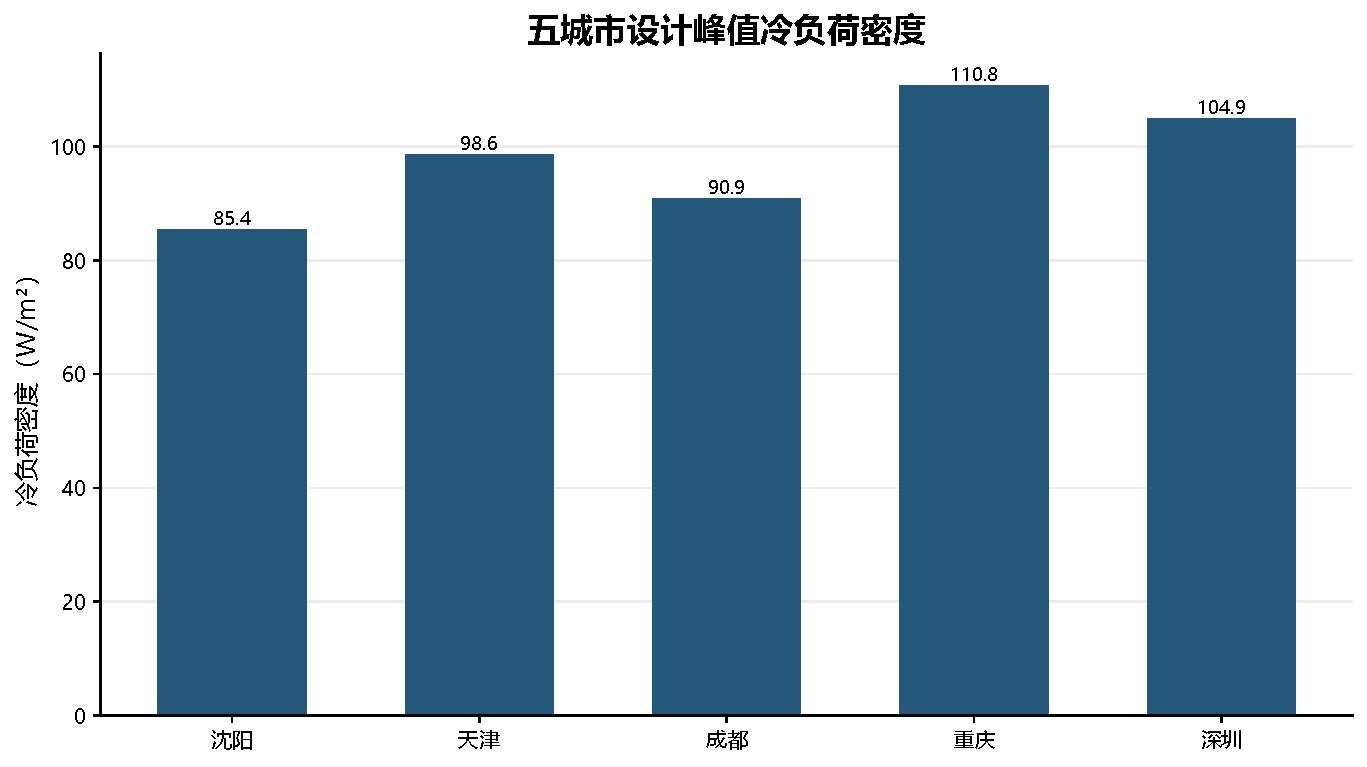
\includegraphics[width=0.9\textwidth]{peak_cooling_load_density_by_city.pdf}
\caption{五城市理想负荷基线下的峰值冷负荷密度比较}
\label{fig:peak-compare}
\end{figure}

\begin{figure}[htbp]
\centering
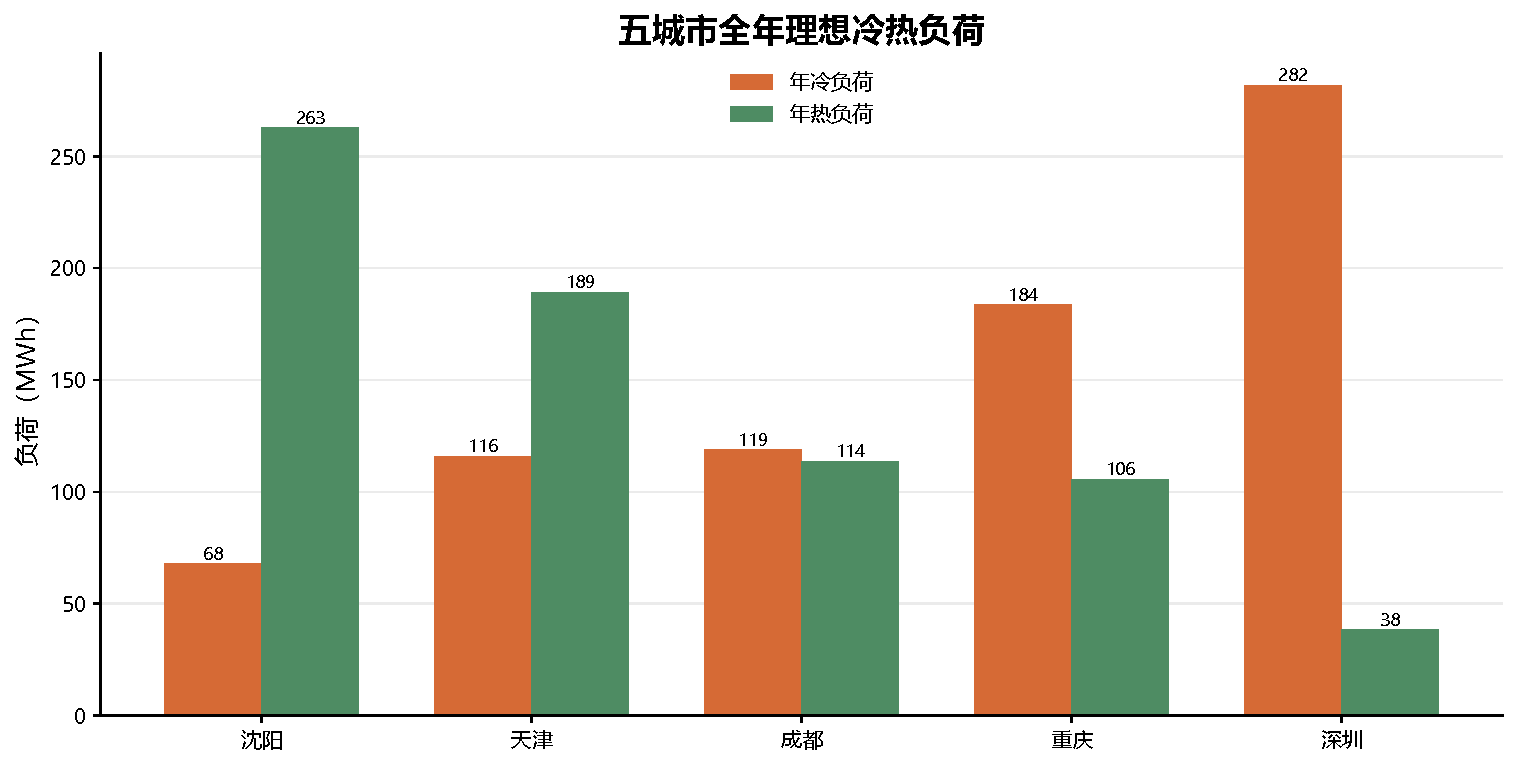
\includegraphics[width=0.9\textwidth]{annual_ideal_loads_by_city.pdf}
\caption{五城市年冷负荷与年热负荷比较}
\label{fig:annual-compare}
\end{figure}

由表\ref{tab:load-comparison}及图\ref{fig:peak-compare}、图\ref{fig:annual-compare}可见，五城市的冷热负荷随气候分区呈现出系统性的梯度变化。

峰值冷负荷方面，天津最高（\SI{17.05}{\kilo\watt}）、深圳次之（\SI{15.74}{\kilo\watt}）、沈阳最低（\SI{10.00}{\kilo\watt}）。天津的峰值冷负荷高于深圳，反映天津夏季较高的室外干球温度（\SI{33.9}{\degreeCelsius} vs \SI{33.7}{\degreeCelsius}）是峰值冷负荷的更强驱动力，而深圳的制冷负荷优势主要体现在全年持续时间而非瞬时峰值。值得注意的是，年冷负荷的排序与峰值冷负荷并不完全一致：深圳年冷负荷最高（\SI{27080}{\kilo\watt\hour}），重庆次之（\SI{19114}{\kilo\watt\hour}），与深圳全年制冷季明显更长这一事实一致。天津年冷负荷（\SI{13486}{\kilo\watt\hour}）在五城市中仅排第四，说明天津虽峰值冷负荷突出，但全年实际制冷运行时长远不及南方城市。

年热负荷方面，从北向南递减：沈阳（\SI{203489}{\kilo\watt\hour}）$ > $ 天津（\SI{169458}{\kilo\watt\hour}）$ > $ 成都（\SI{92799}{\kilo\watt\hour}）$ > $ 重庆（\SI{87752}{\kilo\watt\hour}）$ > $ 深圳（\SI{86479}{\kilo\watt\hour}）。成都、重庆和深圳三者的年热负荷非常接近（约$86$--$93 \times 10^3$ \si{\kilo\watt\hour}），表明在南方三大城市中，空调供热需求已趋于收敛到一个共同的基准水平。与此形成对比，在引入差异化围护结构设计后，沈阳与南方城市之间的热负荷差异达2.4倍（由之前的2.1倍扩大到2.4倍），体现了气候差异在针对性设计下的合理反映。

年总单位面积负荷方面，沈阳最高（\SI{232.95}{\kilo\watt\hour\per\square\meter}），天津次之（\SI{200.74}{\kilo\watt\hour\per\square\meter}），成都最低（\SI{115.47}{\kilo\watt\hour\per\square\meter}）。成都和重庆两座夏热冬冷城市的总负荷强度十分接近（约\SI{116}{\kilo\watt\hour\per\square\meter}），但深圳（\SI{124.60}{\kilo\watt\hour\per\square\meter}）较之高出约7\%，反映了深圳终年维持室内设计温度所需的综合制冷总时数更长。

\subsubsection{影响冷负荷差异的因素分析}

影响空调冷负荷的因素可大致分为两类：与气象有关的因素和与气象无关的因素。在本设计中，与气象无关的因素——室内设计参数（温度、湿度、人员密度、设备及照明功率密度）在五个城市中均设置为同一数值（参见第一章表\ref{tab:indoor-params}），因此各城市间的负荷差异可主要归结为与气象参数相关的因素，包括但不限于室外干球温度、室外湿球温度、太阳辐射强度以及围护结构的传热边界条件。以下从室内冷负荷和新风冷负荷两个维度进行分析。

\textbf{一、室内冷负荷差异}

室内冷负荷主要受围护结构传热和透过外窗的太阳辐射得热影响。在本设计中，围护结构的传热系数在五城市间统一设定，因此室内冷负荷的差异主要来自各城市室外气象参数（尤其是逐时干球温度和外窗得热量）的差异。从表\ref{tab:load-comparison}可以看出，深圳、重庆等全年高温城市的峰值冷负荷高于沈阳等北方城市，这与较高的室外设计温度导致更大的围护结构传热温差直接相关。天津峰值冷负荷突出的现象则提示，峰值冷负荷的高低不仅取决于年平均温度，还与某些极端设计日的气象条件密切相关。

\textbf{二、新风冷负荷差异}

新风冷负荷与室内外空气焓差直接相关。在室内设计温湿度统一的前提下，新风冷负荷的差异主要来自于各城市室外空气的温湿度水平。由图\ref{fig:annual-compare}中各地年冷负荷的差异趋势可以看出，深圳、重庆等高温高湿城市的年冷负荷显著高于北方城市——深圳年冷负荷（\SI{27080}{\kilo\watt\hour}）约为沈阳（\SI{8814}{\kilo\watt\hour}）的3.1倍。即使同属夏热冬冷地区，重庆的年冷负荷（\SI{19114}{\kilo\watt\hour}）也明显高于成都（\SI{12437}{\kilo\watt\hour}），两者之间的差异主要可归因于重庆夏季更高的室外湿球温度（\SI{27.6}{\degreeCelsius} vs \SI{26.4}{\degreeCelsius}）和日平均温度（\SI{30.7}{\degreeCelsius} vs \SI{27.8}{\degreeCelsius}）。

\subsection{系统能耗与设备容量对比}

\subsubsection{年空调电耗强度比较}

表\ref{tab:system-comparison}汇总了五城市两类实际系统的全部比较指标。

\begin{table}[tbp]
\centering
\caption{五城市两类系统比较结果汇总（各系统均设10分区/末端，新风量0.783\,m$^3$/s）}
\label{tab:system-comparison}
\scriptsize
\begin{tabular}{@{}llcccc@{}}
\toprule
\multirow{2}{*}{城市} & \multirow{2}{*}{系统} & \multicolumn{2}{c}{设计容量 (\si{kW})} & \multirow{2}{*}{\makebox[4em][c]{$I_{\mathrm{elec}}$}} & \multirow{2}{*}{\makebox[4em][c]{天然气}} \\
\cmidrule(lr){3-4}
 & & \makebox[3em][c]{冷量} & \makebox[3em][c]{热量} & \si{kWh/m^2} & \si{kWh/m^2} \\
\midrule
沈阳 & VRF+DOAS & 35.60 & 35.60 & 60.25 & --- \\
 & FCU+DOAS & 54.71 & 57.38 & 4.89 & 93.33 \\
\midrule
天津 & VRF+DOAS & 41.70 & 41.70 & 60.20 & --- \\
 & FCU+DOAS & 73.79 & 47.56 & 4.81 & 77.03 \\
\midrule
成都 & VRF+DOAS & 45.80 & 45.80 & 48.85 & --- \\
 & FCU+DOAS & 56.70 & 50.16 & 4.64 & 74.81 \\
\midrule
重庆 & VRF+DOAS & 46.48 & 46.48 & 48.06 & --- \\
 & FCU+DOAS & 96.70 & 39.47 & 5.10 & 74.96 \\
\midrule
深圳 & VRF+DOAS & 54.25 & 54.25 & 56.20 & --- \\
 & FCU+DOAS & 111.74 & 40.42 & 5.67 & 45.10 \\
\bottomrule
\end{tabular}
\end{table}

\begin{figure}[htbp]
\centering
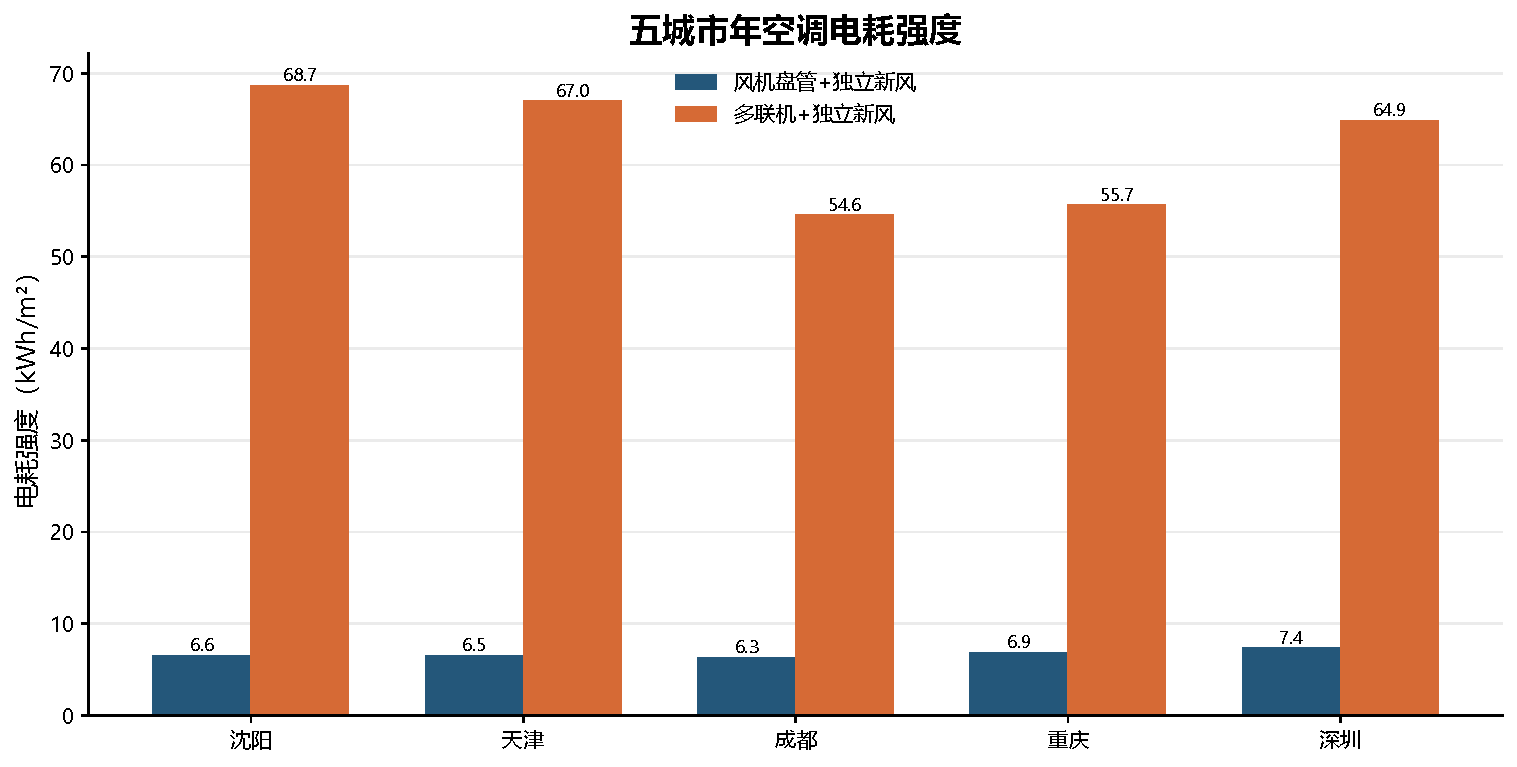
\includegraphics[width=0.9\textwidth]{system_electricity_per_m2_by_city.pdf}
\caption{五城市中VRF+DOAS与FCU+DOAS的年空调电耗强度对比}
\label{fig:elec-compare}
\end{figure}

从图\ref{fig:elec-compare}可以看出：

（1）VRF+DOAS的年空调电耗强度呈现北部城市高于南部城市的总体趋势：沈阳（\SI{60.25}{\kilo\watt\hour\per\square\meter}）$ > $ 天津（\SI{60.20}{\kilo\watt\hour\per\square\meter}）$ > $ 深圳（\SI{56.20}{\kilo\watt\hour\per\square\meter}）$ > $ 成都（\SI{48.85}{\kilo\watt\hour\per\square\meter}）$ > $ 重庆（\SI{48.06}{\kilo\watt\hour\per\square\meter}）。这一梯度与供暖需求的地理分布基本一致。北方VRF系统在冬季需以热泵模式长时间运行，低温工况下性能系数（COP）显著偏低，导致全年压缩机耗电量大幅上升。南方VRF系统虽以制冷为主，全年运行时段长，但制冷工况下VRF的能效比（EER）通常远高于热泵工况下的性能系数（COP），加上南方冬季供热需求较低、热泵总运行时长有限，使全年电耗反而低于北方。

（2）在仅统计空调电耗的当前口径下，FCU+DOAS的年电耗强度（\SI{4.64}{\kilo\watt\hour\per\square\meter}至\SI{5.67}{\kilo\watt\hour\per\square\meter}）在五城市中均显著低于VRF+DOAS。这一差异的核心原因在于，锅炉是FCU+DOAS系统的主要供热设备，其消耗的天然气燃料并未纳入电耗统计。FCU+DOAS的电耗主要由冷水机组、冷却塔风机、冷冻水/热水循环泵及DOAS送风机等电力设备贡献。本研究通过提取并解析EnergyPlus系统底层报告，成功补齐了FCU+DOAS系统的全年天然气消耗总量。结果显示，各城市的年天然气消耗量分别为：沈阳\SI{127574.93}{\kilo\watt\hour}（折合强度\SI{93.33}{\kilo\watt\hour\per\square\meter}）、天津\SI{105295.70}{\kilo\watt\hour}（折合强度\SI{77.03}{\kilo\watt\hour\per\square\meter}）、%
成都\SI{102261.53}{\kilo\watt\hour}（折合强度\SI{74.81}{\kilo\watt\hour\per\square\meter}）、重庆\SI{102472.47}{\kilo\watt\hour}（折合强度\SI{74.96}{\kilo\watt\hour\per\square\meter}）%
和深圳\SI{61653.32}{\kilo\watt\hour}（折合强度\SI{45.10}{\kilo\watt\hour\per\square\meter}）。可以看出，天然气消耗强度随着气候供暖需求的降低而显著下降。

（3）两种系统在五城市间的电耗波动幅度差异显著：VRF电耗强度的极差（最大值减最小值）为\SI{12.19}{\kilo\watt\hour\per\square\meter}，而FCU电耗强度的极差仅为\SI{1.03}{\kilo\watt\hour\per\square\meter}。这表明VRF系统的电耗对气候条件的敏感度远高于FCU+DOAS系统的"电耗"部分——这与VRF的直膨式压缩机直接响应室外气温和室内负荷变化有关，而FCU冷水机组的运行主要取决于供冷侧需求，供热侧电耗则因锅炉的存在而基本为零。

\subsubsection{设备设计容量比较}

\begin{figure}[htbp]
\centering
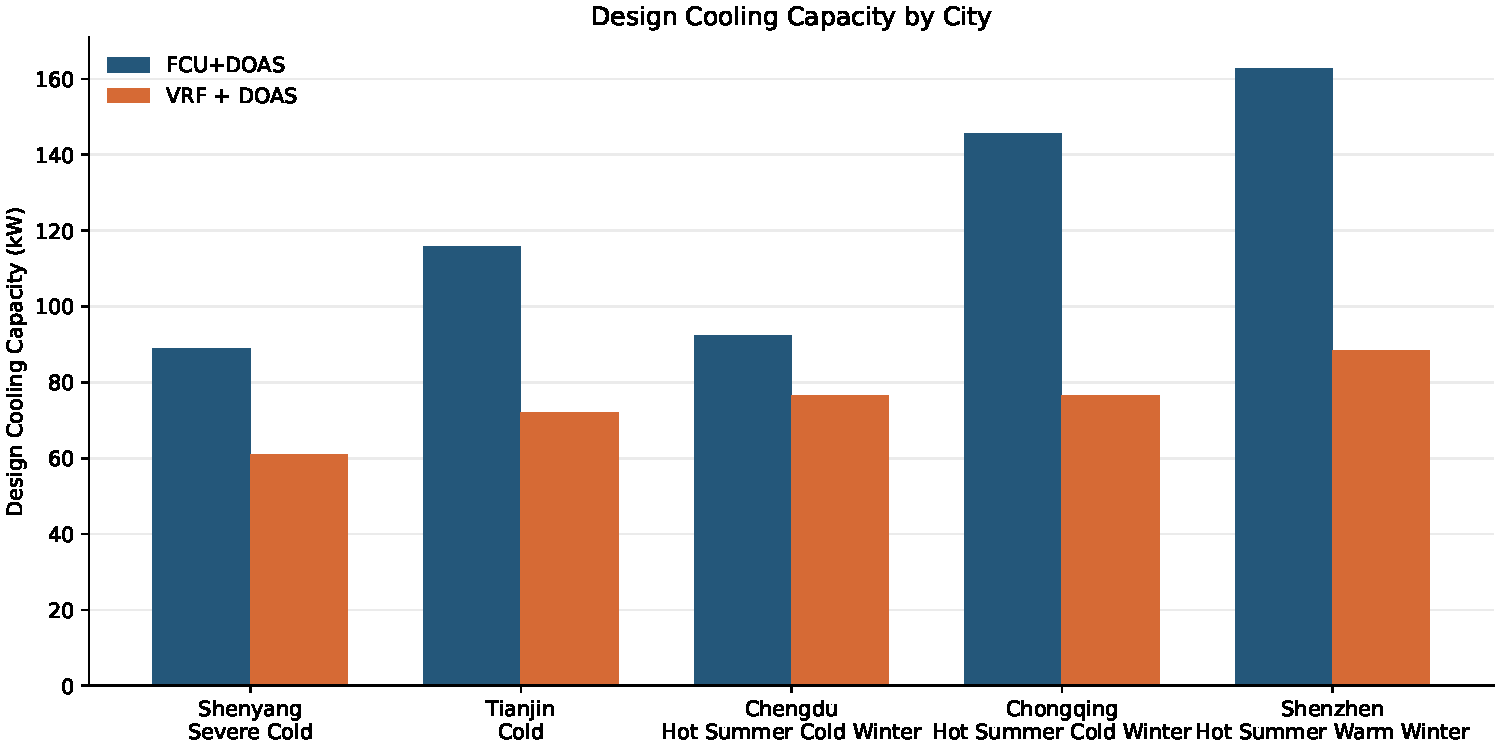
\includegraphics[width=0.9\textwidth]{design_cooling_capacity_by_city.pdf}
\caption{五城市两类系统的设计冷量比较}
\label{fig:capacity-compare}
\end{figure}

由图\ref{fig:capacity-compare}可得出以下规律：

（1）VRF方案的设计冷量由北向南递增，从沈阳\SI{35.60}{\kilo\watt}到深圳\SI{54.25}{\kilo\watt}，%
极差为\SI{18.65}{\kilo\watt}。各城市VRF冷热共用同一台热泵室外机，设计冷量与设计热量相等，因此该方案在满足制冷需求的同时也自动提供了等额的供热容量。

（2）FCU方案中，冷水机组设计冷量随制冷需求从沈阳\SI{54.71}{\kilo\watt}增加至深圳\SI{111.74}{\kilo\watt}，各城市间的差异远大于VRF方案。FCU冷水机组设计冷量普遍高于同城市的VRF设计冷量，差异幅度从\SI{10.90}{\kilo\watt}（成都）至\SI{57.49}{\kilo\watt}（深圳）不等。这反映出集中冷源在自动选型时倾向于保留更大的设计余量，且该余量在不同城市间表现出明显差异。

（3）FCU方案中锅炉设计热量在沈阳最高（\SI{57.38}{\kilo\watt}），其次为成都（\SI{50.16}{\kilo\watt}）、天津（\SI{47.56}{\kilo\watt}）、深圳（\SI{40.42}{\kilo\watt}）和重庆（\SI{39.47}{\kilo\watt}），与年热负荷的地理分布高度吻合。沈阳FCU的锅炉设计热量为重庆的1.45倍，反映了严寒地区与夏热冬冷地区在供热容量配置上的合理差异。

\subsection{技术方案适宜性评价}

综合上述跨城市、跨系统的对比分析，本节从以下几个方面对两类方案在不同气候分区的技术适宜性进行评价。

\subsubsection{系统运行效率与气候适配性}

VRF+DOAS方案的核心优势在于系统的简洁性与灵活调节能力：一台室外机通过制冷剂管路连接10台室内末端，无需建设集中的冷冻水和热水系统，设备占用空间小，系统环路控制相对简单\cite{liu2010vrf_gshp,kanisanchez2017vrf_whole_building}。然而，对该方案而言，其全年运行的经济性和能效高度依赖于室外气象条件：在深圳这样以制冷为主的城市，VRF以较高能效比（EER）运行，年电耗强度降至\SI{56.20}{\kilo\watt\hour\per\square\meter}；在沈阳这样冬季严寒的城市，VRF热泵在低温工况下性能系数（COP）下降明显\cite{aynur2010vrf_desiccant}，全年电耗显著上升。

FCU+DOAS方案的核心优势在于冷热源分离：冷水机组供冷、燃气锅炉供热，各自在设计的温度范围内以较高的设备效率运行\cite{kim2016vrf_doas_control}。然而，FCU+DOAS需要设置集中冷热站、冷却塔、冷冻水与热水双管路系统，系统组成复杂度显著高于VRF方案。本课程设计的关键发现之一是：在仅统计电耗的情况下，FCU+DOAS的电耗极低，但这一指标掩盖了锅炉燃气消耗的实际占比\cite{wang2023hscw_heating}。因此，FCU+DOAS的完整技术适宜性评价仍有待合并天然气消耗之后。

\subsubsection{设备容量配比与建筑负荷的匹配}

从室内外机容量配比的角度来看（参照参考课程设计关于VRF机组组合率应在50\%--130\%范围内的分析逻辑），本文五个城市的VRF方案中，一台室外机连接10台室内末端，室外机设计冷量范围\SI{35.60}{\kilo\watt}至\SI{54.25}{\kilo\watt}，各分区的末端容量合计约为室外机容量的100\%--130\%，基本遵循了机组组合率的推荐范围。各城市VRF配比率基本一致，说明在相同的建筑分区和负荷分布下，VRF系统在不同气候分区间保持了较为稳定的容量匹配关系。

FCU+DOAS方案中，冷水机组设计冷量与锅炉设计热量的比值随气候冷暖特征变化呈现显著梯度：沈阳0.95:1、成都1.13:1、天津1.55:1、重庆2.45:1、深圳2.76:1。这一比值本身即可作为气候分区的一个定量化标识——比值接近1.0表明该城市供冷与供暖高峰负荷并重（严寒地区），比值大于2.5则表明以绝对制冷需求为主导（夏热冬暖及湿热的夏热冬冷地区）。

\subsubsection{综合评价与选型建议}

在统一建筑原型和统一输入边界的条件下，本文的比较结果支持以下初步判断：

（1）对于沈阳和天津所代表的寒冷及严寒地区，FCU+DOAS方案通过集中锅炉与冷水机组分别处理冷热需求，在容量配置上具有更高的灵活性，但需要关注锅炉燃料消耗带来的运行费用和碳排放。VRF+DOAS方案在严寒地区以较高的年电耗为代价换取了系统简洁性，是否优先选用取决于用户对投资成本、运行费用和系统管理复杂度的综合权衡。

（2）对于成都、重庆和深圳所代表的夏热冬冷及夏热冬暖地区，VRF\kern0pt+DOAS方案在制冷主导的全年运行模式下表现出更好的电力经济性（年电耗强度较北方降低18\%--20\%），且系统简洁性的优势在南方较短的供暖季中更为突出。

（3）重庆作为夏热冬冷地区中高温高湿特征最为突出的城市，其FCU冷水机组设计冷量（\SI{96.70}{\kilo\watt}）为五城市中次高（仅次于深圳\SI{111.74}{\kilo\watt}），而VRF设计冷量为\SI{46.48}{\kilo\watt}。重庆FCU冷水机组选型容量显著偏高的现象提示，该城市在采用集中冷源方案时，自动选型算法可能因夏季极端设计日的湿球温度较高而显著放大了设计冷量需求。因此，在重庆等高温高湿城市中，FCU方案在设计阶段应特别关注冷水机组选型的合理性和备用容量设定，避免设计冷量过度安全。

\subsubsection{当前评价的限定条件}

本设计的适宜性评价存在若干明确的限定条件，需要在结论解读时予以说明。第一，本研究已按GB~50189-2015实现了围护结构（外墙、屋面保温厚度）的差异化设定，但外窗传热系数和窗墙比等参数在当前五城市中仍保持统一，尚未进行更细致的分区窗型优化（例如北方严寒地区使用更低传热系数的三玻窗或Low-E窗）。第二，虽然本研究通过提取并解析EnergyPlus系统底层报告成功补齐了FCU+DOAS系统的年天然气消耗总量，但当前的系统能耗比较尚未统一转换为一次能源（标煤）或全生命周期碳排放指标，使得两种异质能源（电耗与燃气消耗）的对比仍显分离。第三，本课程设计未涉及初投资、运行维护费用和全生命周期经济性分析，因此本文的适宜性评价主要着眼于技术指标层面，尚未上升到全口径经济性比较层面。

\section{总结}

本课程设计以三层办公楼为工程对象，建筑面积约\SI{1358.4}{m^2}，平面尺寸约\SI{32.0}{m} $\times$ \SI{14.15}{m}。在参考论文设计思路基础上，本文保留房间级热源参数、冷负荷逐时叠加、末端设备选型和施工图校核的基本流程，同时将建筑扩展为三层，并增加重庆城市分支。计算与绘图均围绕天正暖通设计流程展开：平面图采用黑白CAD出图风格，负荷计算采用CLTD/CLF思路，设备表按房间峰值冷负荷、标准容量档位和楼层组合率生成。

本研究的主要结论如下：

第一，五城市峰值冷负荷为\SI{116.07}{kW}--\SI{150.48}{kW}，冷负荷密度为\SI{85.4}{W/m^2}--\SI{110.8}{W/m^2}。重庆峰值最高，为\SI{150.48}{kW}；深圳为\SI{142.54}{kW}，虽然低于重庆，但供冷季更长；沈阳为\SI{116.07}{kW}，仍需按设计日完成新风和末端冷量校核。

第二，全楼按50个房间设置人员、照明、设备和新风参数，其中47个房间纳入空调服务。设计人数为187人，基准新风量为\SI{7250}{m^3/h}。五城市新风负荷为\SI{46.42}{kW}--\SI{70.55}{kW}，占全楼峰值冷负荷39.6\%--46.9\%。重庆和深圳的新风除湿负荷最突出，DOAS盘管冷量、送风露点和冷凝水排放应作为施工图阶段的重点校核项。

第三，围护结构按城市气候区进行差异化设计。沈阳和天津采用较低的外墙、屋面传热系数；成都、重庆和深圳采用更强的外窗遮阳控制，其中深圳外窗传热系数取\SI{2.20}{W/(m^2\cdot K)}、遮阳系数取0.33。灵敏度分析表明，新风量是影响设备容量的首要参数，30/50~m$^3$/(h$\cdot$人)扰动可使峰值冷负荷变化约9.9\%--11.7\%；窗墙比和设备功率密度次之，围护结构增强和遮阳优化可提供小幅但稳定的容量下降。

第四，VRF+DOAS方案按房间峰值冷负荷乘1.3安全系数选取室内机，三层共配置47--48台室内机；各城市室内机总容量为\SI{200.1}{kW}--\SI{243.1}{kW}，室外机总容量为\SI{174.0}{kW}--\SI{209.5}{kW}，楼层组合率控制在107.7\%--117.9\%。该结果说明房间末端选型、全楼同时峰值和楼层室外机容量不能互相替代，必须分别校核。

综合来看，沈阳适合强调短时峰值和低负荷稳定，天津与成都两类系统均具备可行性，重庆和深圳应优先保证DOAS除湿和长供冷季运行可靠性。本文的核心价值不在于复刻参考论文的具体数值，而在于形成一套可迁移的制冷空调设计流程：黑白CAD平面图确定房间边界，天正暖通房间级参数确定冷负荷，五城市围护结构体现地域差异，设备选型表落实到末端和楼层系统，灵敏度分析用于识别后续施工图最需要复核的设计输入。

\appendix
\section{可复现性说明}

本文所有数值结果均直接来源于EnergyPlus仿真输出的统一整理结果。论文中的图表与表格保持同一数据来源，以确保比较逻辑和结论表述的一致性。本文所依托的数据与代码均已开源发布于：\url{https://github.com/twj0/air-conditioning-design}，可用于后续复核、扩展和进一步写作。

当前论文版本在结论表达上保持审慎。文中已明确区分“空调电耗口径比较”与“完整系统综合能耗比较”之间的差异。对于FCU+DOAS方案，现阶段结果尚未纳入锅炉燃料消耗，因此相关比较主要反映其电耗表现而非全口径能耗表现。此外，五城市当前采用统一围护结构参数，尚未按GB~50189-2015对不同气候分区进行围护结构差异化设计，这一限制在第七章已作讨论。

\section*{作者贡献声明}

作者信息由论文提交时补充填写。本文现阶段稿件的主要工作包括模型建立、结果整理、图表生成、结果分析与论文撰写。

\section*{数据与代码可用性}

本文相关数据与代码已开源发布于：\url{https://github.com/twj0/air-conditioning-design}。

\section*{利益冲突声明}

作者声明不存在可能影响本文研究结论的利益冲突。

\section*{致谢}

感谢课程设计任务背景、公开气象数据资源以及EnergyPlus参考模型为本文工作提供基础条件。


\bibliographystyle{cls/elsarticle-num}
\bibliography{bib/references}

\end{document}
